%
% Extensive description of the document; history, table of the acronyms
%
% Author:
% Version:
%
\subsection[Prologue]{Prologue}
\label{Prologue}
The first generation of interferometric gravitational wave (GW) detectors (GEO600~\cite{GEO600Grote2008}, LIGO~\cite{Abbott2009}, TAMA~\cite{Arai2008}, Virgo~\cite{VirgoStatus2008}) have reached or approached their design sensitivities, and thus demonstrated the effectiveness of the working principle. The major detectors currently operative are enhanced versions of the first generation (Virgo+ and E-LIGO), with higher laser power and some technological improvements. \par
Advanced detectors (like ``Advanced LIGO" and ``Advanced Virgo"), which are also called the second generation, will show a sensitivity improved roughly by a factor of ten with respect to the initial interferometers. They are based on technologies currently available, sometimes tested in reduced scale prototypes, but still to be implemented in full scale. According to the current models of GW sources, the sensitivity of the advanced interferometers is expected to guarantee the detection of the signals generated by astro-physical sources within months to a year at most. For example, at the nominal sensitivity of the advanced detectors, the expected detection rate of the GW signal generated by a binary system of coalescing neutron stars is about a few tens per year. But apart from extremely rare events, the expected signal-to-noise ratio (SNR) of these detections obtained with the advanced detectors is too low for precise astronomical studies of the GW sources and for complementing optical and X--ray observations in the study of fundamental systems and processes in the Universe. \par
These considerations led the GW community to start investigating a new (third) generation of detectors. In particular, the European Commission supported the institutions in table~\ref{table:Beneficiaries} to realise this design study within the Seventh Framework Programme (FP7-Capacities). With a considerably improved sensitivity these new machines of the third generation will open the era of routine GW astronomy and with the Einstein Telescope (ET) project Europe will lead this scientific revolution. Since the first detection of a GW signal is expected to occur in the advanced interferometers, the evaluation of the scientific impact of ET it is especially focused on the observational aspects rather than on the detection capabilities. \par
\nomenclature[aET]{ET}{Einstein Telescope}
To realise a third generation GW observatory with a significantly enhanced sensitivity (we defined a target of a factor of ten improvement in sensitivity for ET with respect to the advanced detectors over a wide frequency range), several limitations of the technologies adopted in the advanced interferometers must be overcome and new solutions to be developed are proposed in this document to reduce the fundamental and technical noises that will limit the next generation machines. \par
However, the first and main target of this document is the definition of the requirements and of the main characteristics of the site hosting ET, the design of the key elements of the research infrastructure, the rough evaluation of the costs and of the timeline of its implementation.  To understand the importance and the need of the site and infrastructures in the ET design it is worth to recall the history of the current GW detector infrastructures, shown in Fig.~\ref{Fig:InfraEvolution}; current and advanced detectors are using the same infrastructure that will be about 20 years old when the second generation will be online. Any further improvement of the sensitivity will be limited by the constraints of the site and infrastructure (arm length, local seismic noise, absence of cryogenic apparatus, vacuum pipe size, \dots). On the contrary, in order to realise a third-generation GW observatory like ET, an infrastructure  hosting several detectors evolving for many decades is crucial.
%

\begin{table}[ht]
% For LaTeX tables use
\centering
\begin{tabular}{c|c}
\hline
\hline
Institute & Country   \\
\hline \hline
European Gravitational Observatory & Italy--France \\
\hline
Istituto Nazionale di Fisica Nucleare & Italy \\
\hline
Max-Planck-Gesellschaft zur F{\" o}rderung der Wissenschaften e.V., & \\
acting through Max- Planck-Instit{\" u}t f{\" u}r Gravitationsphysik  & Germany \\ \hline
Centre National de la Recherche Scientifique  & France \\
\hline
University of Birmingham & United Kingdom \\
\hline
Glasgow University & United Kingdom \\
\hline
Nikhef & The Netherlands \\
\hline
Cardiff University & United Kingdom \\
\hline
\hline
\end{tabular}
\caption{Institutions participating (``Beneficiaries") to the ET design study}
\label{table:Beneficiaries}       % Give a unique label
\end{table}

To realise a third generation GW observatory with a significantly enhanced sensitivity (we defined a target of a factor of ten improvement in sensitivity for ET with respect to the advanced detectors in a wide frequency range), several limitations of the technologies adopted in the advanced interferometers must be overcome and new solutions to be developed are proposed in this document to reduce the fundamental and technical noises that will limit the next generation machines. \par 
However, the first and main target of this document is the definition of the requirements and of the main characteristics of the site hosting ET, the design of the key elements of the research infrastructure, the rough evaluation of the costs and of the timeline of its implementation.  To understand the importance and the need of the site and infrastructures in the ET design it is worth to recall the history of the current GW detector infrastructures, shown in Fig.~\ref{Fig:InfraEvolution}; current and advanced detectors are using the same infrastructure that will be about 20 years old when the second generation will be online. Any further improvement of the sensitivity will be limited by the constraints of the site and infrastructure (arm length, local seismic noise, absence of cryogenic apparatus, vacuum pipe size, \dots). On the contrary, in order to realise a third-generation GW observatory like ET, an infrastructure  hosting several detectors evolving for many decades is crucial.
%

\begin{figure}
\centering
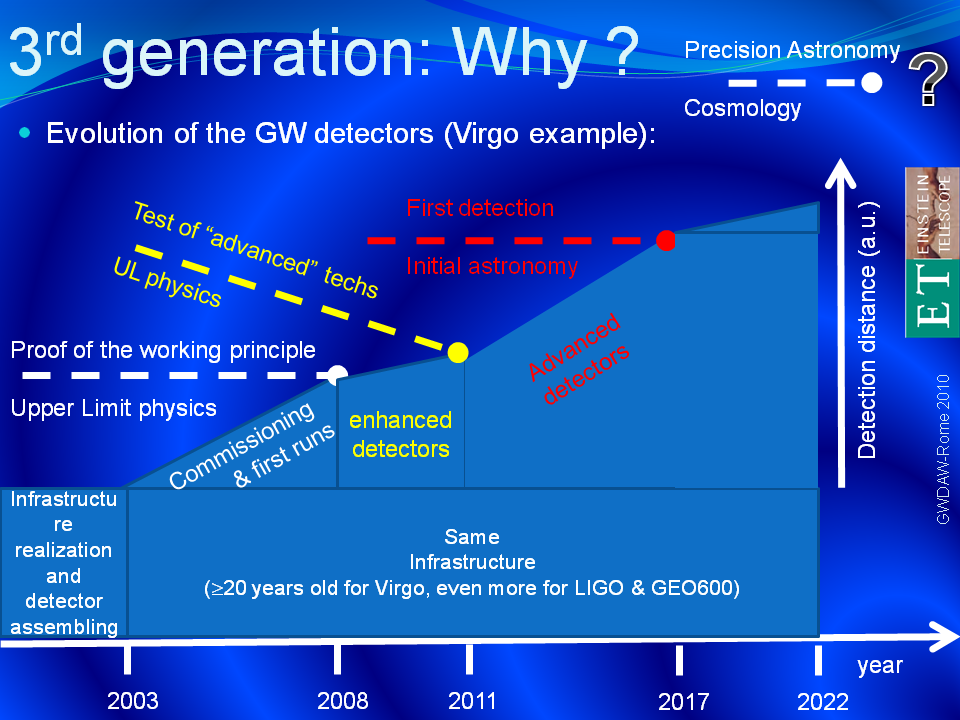
\includegraphics[width=0.9\textwidth]{Sec_Introduction/GWDAW-2010PunturoInfrastructureAdv.png}
%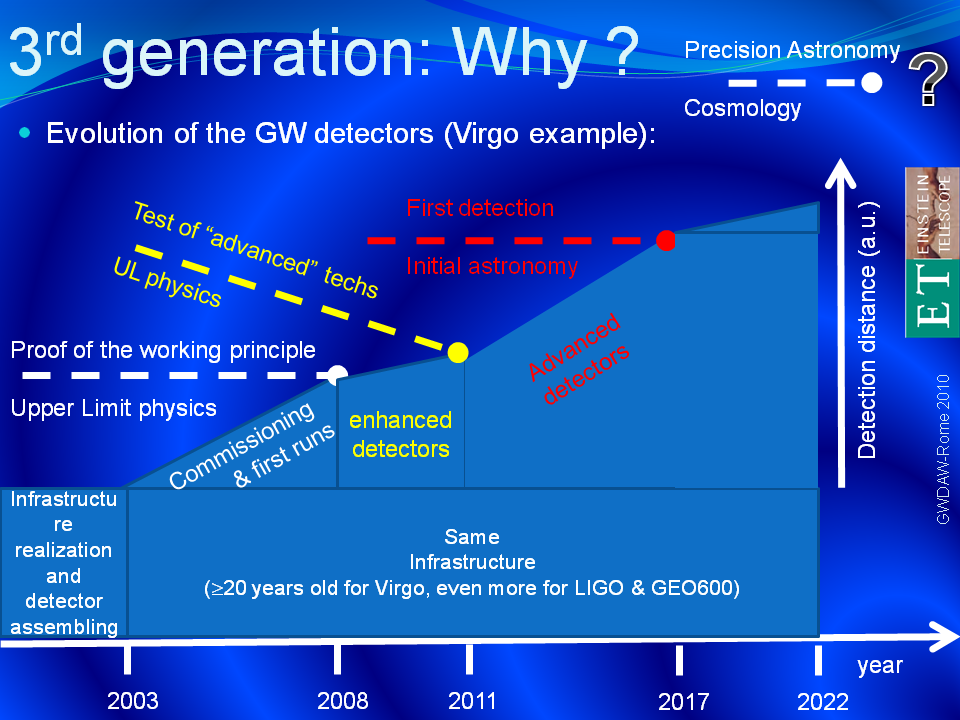
\includegraphics[width=0.9\textwidth, bb=0 0 800 600]{Sec_Introduction/GWDAW-2010PunturoInfrastructureAdv.png}
%\includegraphics[width=0.49\textwidth, bb=0 0 800 600]{ET-B.png}
\caption{Evolution of the first and second generation GW detectors. Time is on the horizontal axis, detector performances in the vertical one. When the advanced detectors will be operative the hosting infrastructures will be more than 20 years old and any further improvement of the performances (sensitivity) will be suppressed by the limitation imposed by the infrastructures. (slide presented by M.\,Punturo at the GWDAW meeting, Rome Jan.\,2010) }
\label{Fig:InfraEvolution}
\end{figure}
%
%
\FloatBarrier

%%%%%%%% box ET in 1 minute
\etbox{h}{ETin1minute}{The Einstein Telescope in one minute reading}{
The \emph{Einstein gravitational--wave Telescope} will be an observatory of the third generation aiming to reach a sensitivity for GW signals emitted by astrophysical and cosmological sources about a factor of 10 better than the advanced detectors currently being built. An observatory with such a level of sensitivity will open the era of routine GW astronomy. \\
An artists impression of the Einstein Telescope is given in figure~\ref{fig:ET_artists_view}. The main purpose of the ET project is the realisation of an infrastructure (an ``observatory"), capable of hosting more than one GW detector. This infrastructure will be usable for many decades, while the implemented detectors will undergo successive upgrades or replacements according to the current state of the art of interferometer technologies. \\
To reduce the effect of the residual seismic motion, which allows a better sensitivity at low frequencies (between 3 and 100\,Hz), ET will be located underground at a depth of about 100 m to 200 m and, in the complete configuration, it will consist of three nested detectors each in turn composed of two interferometers (\emph{xylophone} configuration). The topology of each interferometer will be the dual recycled Michelson layout with Fabry--Perot arm cavities, with a length of about 10~km. The Xylophone configuration of each detector allows to devote one interferometer to the detection of the low frequency components of the GW signal (2--40\,Hz) and to dedicate the other one to the high frequency components, each interferometer adopting different, optimal technologies. In the former one (ET-LF), operating at cryogenic temperature, the thermal, seismic, gravity gradient and radiation pressure noise sources will be particularly suppressed; in the latter one (ET-HF) the sensitivity at high frequencies will be focussed on using  high laser light power circulating in the Fabry--Perot cavities and adopting frequency dependent squeezed light technologies. The target sensitivity of the ET observatory, at the current level of understanding, is shown in figure~\ref{fig:ET_sensitivity}.
}

%%%%%%%% end box ET in 1 minute

%%%%%begin info box on gravitational wave
\etbox{i}{box:detecting_gw}{Detecting Gravitational Waves}{
Gravitational waves change distances between objects with opposing sign for orthogonal directions by changing the metric of space-time, while the objects themselves locally remain at rest, as illustrated in figure~\ref{fig:GWeffect} for one polarisation of the wave ($\rm{h_+}$)(see\,\ref{box:response}).
\begin{figure}[H]
		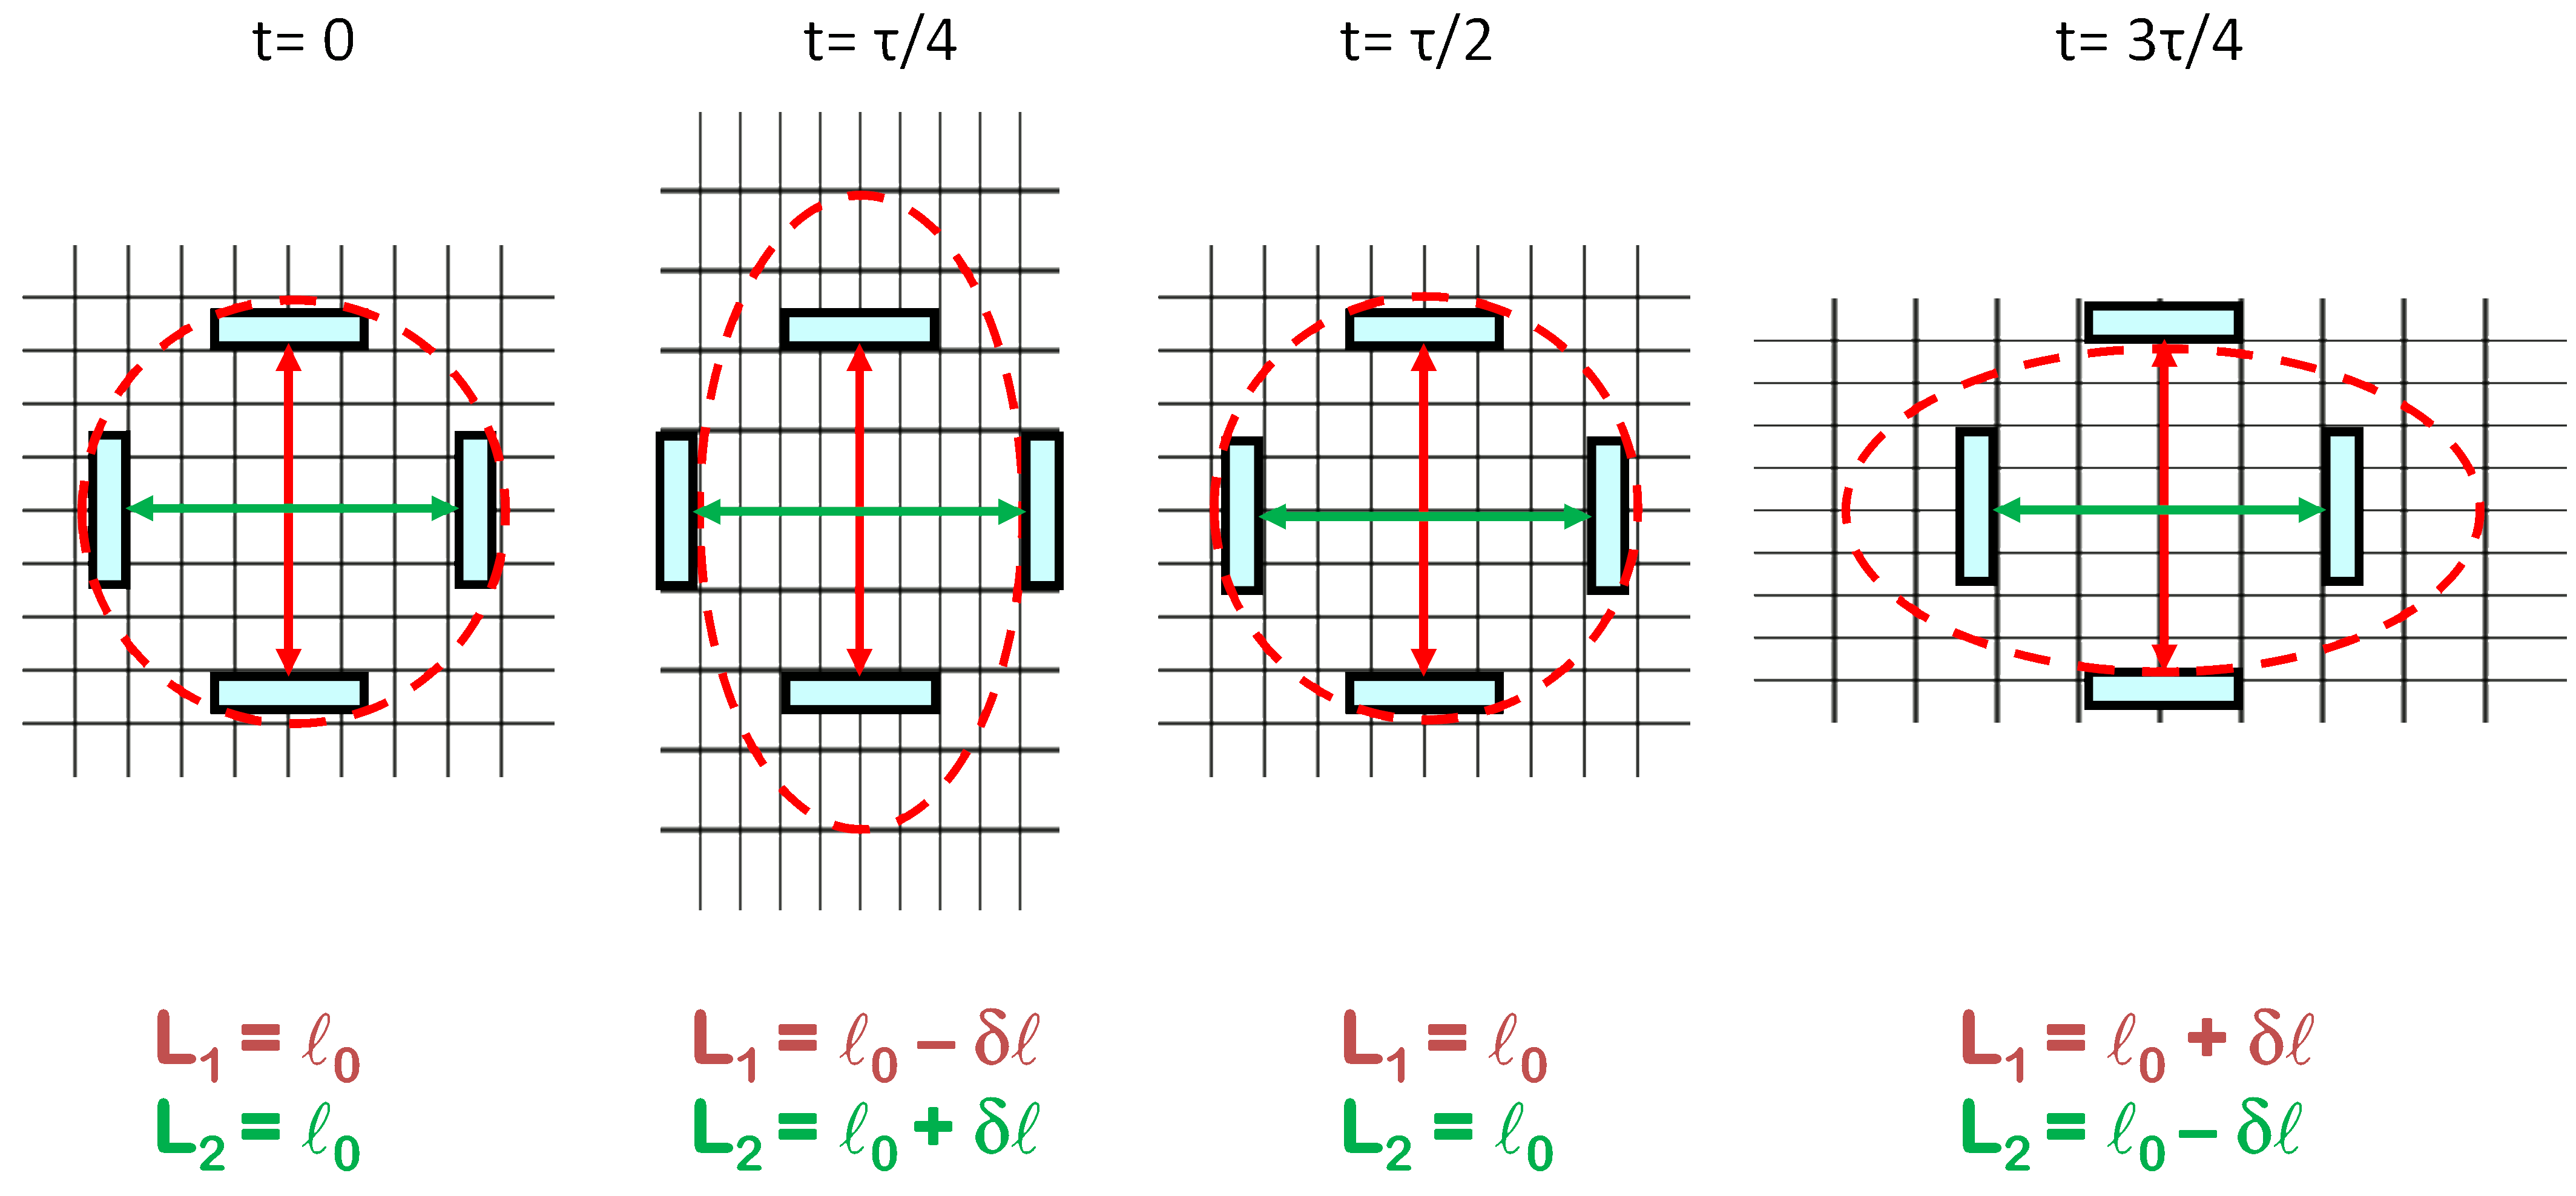
\includegraphics[width=\textwidth]{Sec_Introduction/GWeffect.png}
	\caption{The effect of gravitational waves on the distances of objects. While the mirrors remain locally at rest the metric gets changed by the gravitational wave. The figure shows the effect of a sinusodial gravitational wave with period $\rm{\tau}$, for different times T. The distances measured between the mirrors change by $\pm\delta\,l$.}
	\label{fig:GWeffect}
\end{figure}
For measuring this effect a Michelson interferometer is ideally suited. The measurement principle is shown in figure~\ref{fig:GWdetection}. A laser beam is split into two partial beams, send along the interferometer arms, where it experiences a phase shift by the metric change of the gravitational wave, is reflected at the end and returns to the beamsplitter, where it is recombined. The interference condition at the beam splitter, i.e.\ the phase relation of the two returning beams, determines the intensity on the photo detector. Three different phase relations are shown in figure~\ref{fig:GWdetection}. The relative length change of the interferometer arms can hence be detected by measuring the power at the output port. Although the measurement principle is very simple, for getting the best possible sensitivity all influences that change the geometrical or optical arm length or that cause a signal in the detected photocurrent mimicking a gravitational wave have to be minimised, resulting in very sophisticated and complex instruments.
\begin{figure}[H]
		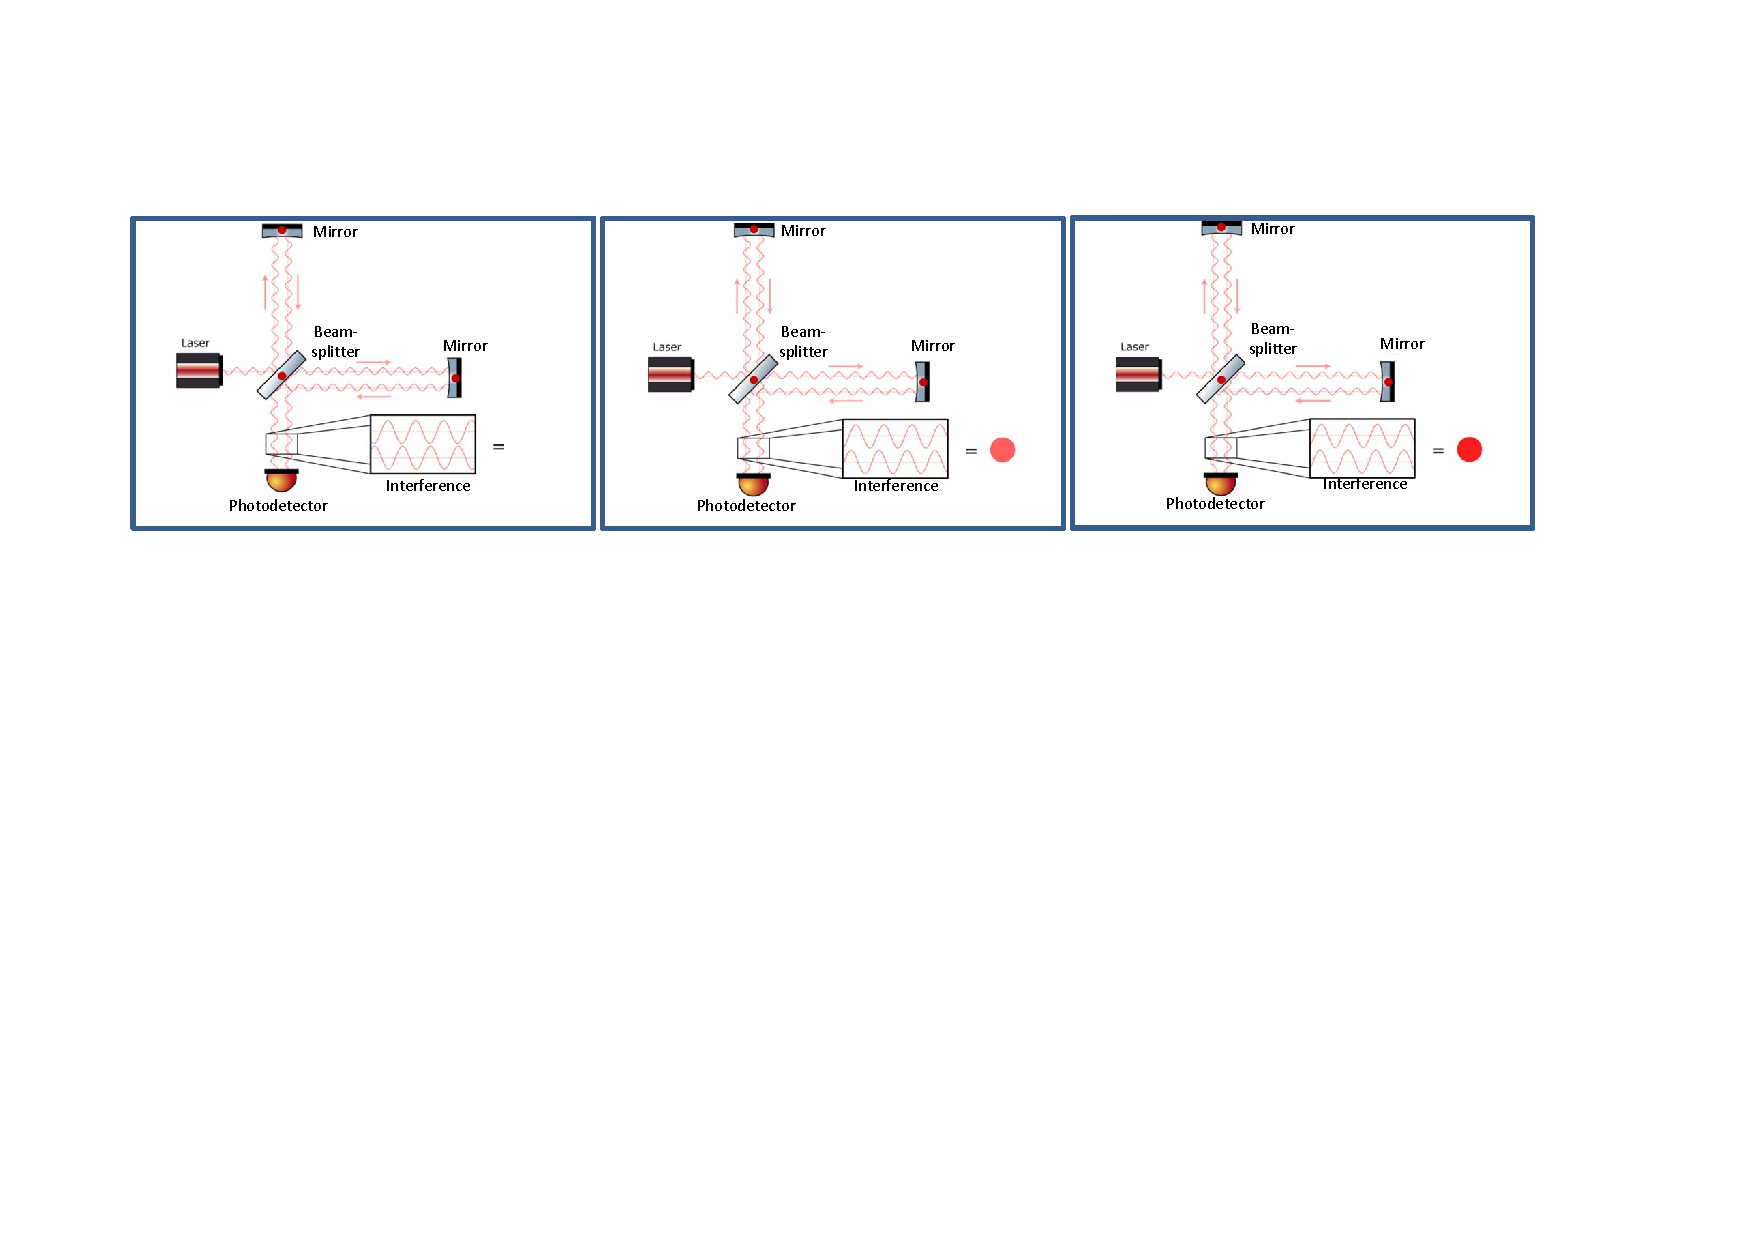
\includegraphics[width=\textwidth]{Sec_Introduction/GWdetection.pdf}
	\caption{Michelson interferometer principle for gravitational wave detection, showing three different interference conditions resulting in different brightness at the output port.}
	\label{fig:GWdetection}
\end{figure}
}

%%%%%end info box on gravitational wave

\begin{figure}[!h]
	\centering	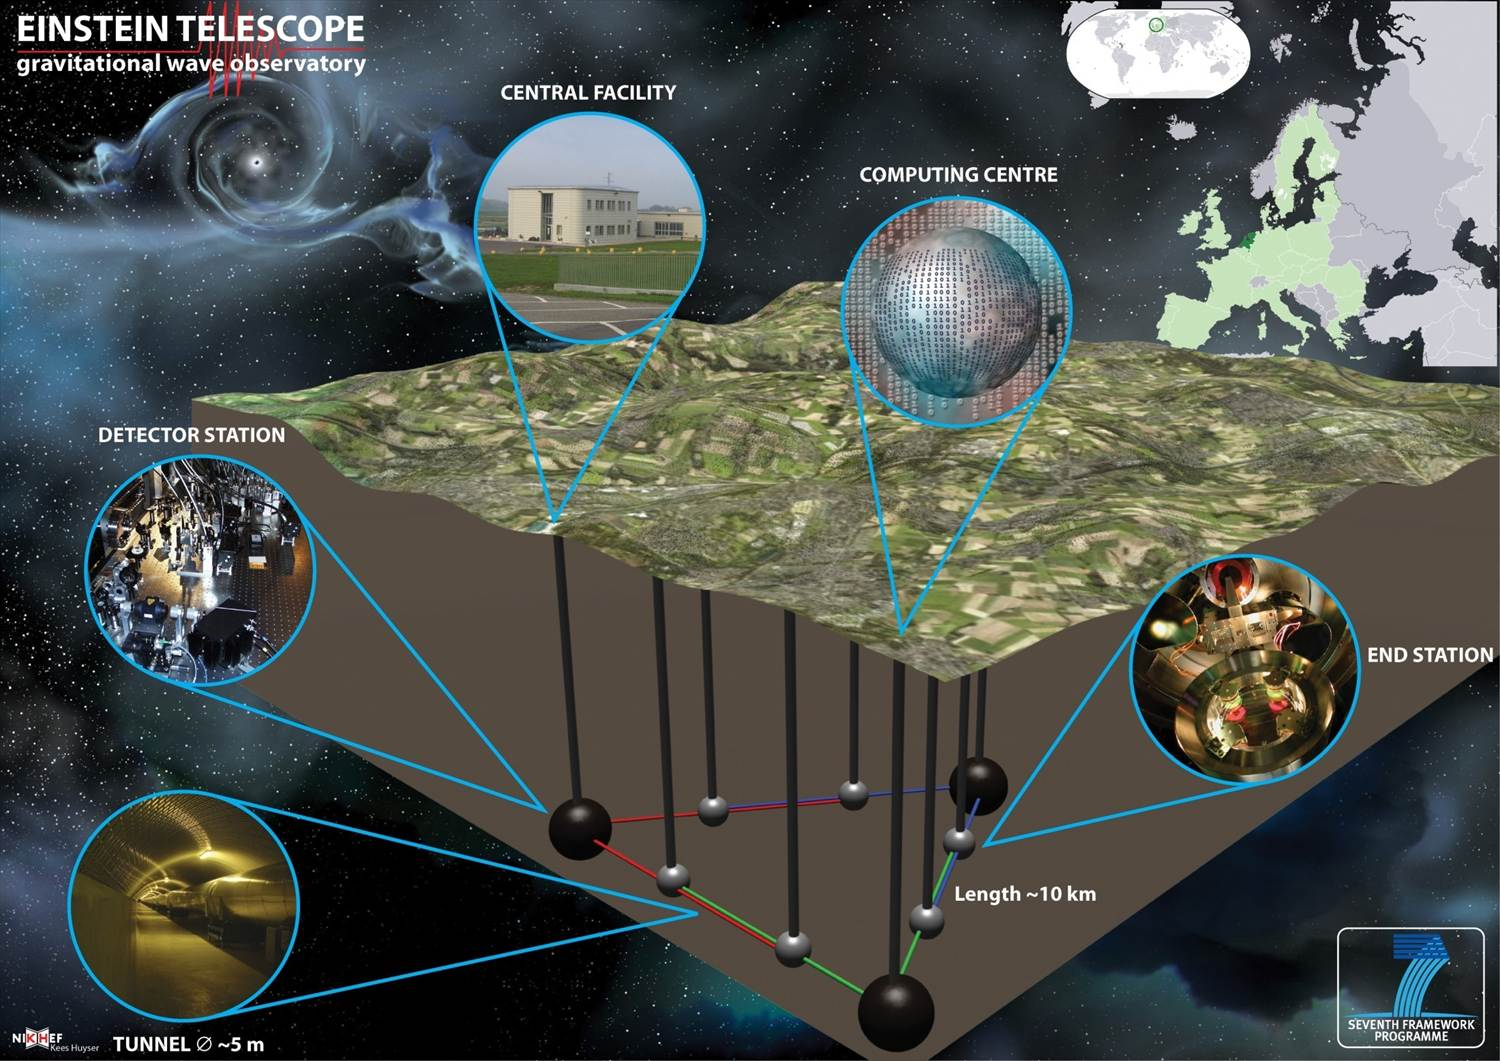
\includegraphics[width=1.00\textwidth]{Sec_Introduction/ET_artists_view.jpg}
	\caption{Artists view of the Einstein Telescope}
	\label{fig:ET_artists_view}
\end{figure}


\FloatBarrier
\subsection{Scientific targets of the ET observatory}
\emph{Authors: M.Punturo, H. Lueck} \\
%put here a short summary of the astrophysical and cosmological  targets of ET. A good fraction of the text could be created cutting and pasting the section~\ref{ScienceCase:FundamentalPhysics} and successive.
\subsubsection{Fundamental physics}
\label{ScienceCase:FundamentalPhysics}
Astronomical sources of gravitational waves are essentially
systems where gravity is extremely strong and often
characterized by relativistic bulk motion of massive objects.
The emitted radiation carries an uncorrupted signature of the
nature of the space-time geometry and so an invaluable
tool to understand the behaviour of matter and geometry in
extreme conditions of density, temperature, magnetic fields
and relativistic motion. Here are some examples of how GW
observations can impact fundamental physics.

In Einstein's theory, gravitational radiation travels at the
speed of light and has two polarization states. In alternative
theories of gravity one or both of these properties might not
hold, owing to the presence of massive gravitons, or a scalar
field mediating gravity in addition to the tensor field. Experimental
tests of gravity, as well those afforded by the data from the
Hulse-Taylor binary, are consistent with both Einstein's theory
and one of its alternatives called the Brans-Dicke theory.
Gravitational wave detectors will bring these theories
vis-a-vis observations that could decisively rule out one
or the other.

According to Einstein's gravity the space-time in the vicinity
of black holes is described by a unique geometry called the
Kerr solution. Observation of the radiation from the in-fall
of stellar-mass black holes into intermediate-mass black holes
will make it possible to test such uniqueness theorems. X-ray
astronomy has provided firm indirect evidence that intense
sources of x-rays may well host a black hole. An unambiguous
signature of the black hole geometry, however, could eventually
be provided by the detection of black hole quasi-normal modes:
gravitational radiation with characteristic frequencies and decay
times that depend only on the mass and spin angular momentum of the black hole.
Failure to detect such radiation from, for example, a newly
formed black hole would mean that gravity is more exotic than
what we currently believe,
%(e.g., gravitational collapse might lead to entities called naked singularities)
and might reveal new phases of matter at extremely high densities.

The most attractive versions of string theory require a ten- or
eleven-dimensional space-time, far larger than what we perceive.
In certain phenomenological models at the interface of string
theory and cosmology, what we perceive as a four-dimensional
Universe could be one part, or ``brane'', within a higher
dimensional ``bulk'' Universe. The extra spatial dimensions may
be compact and sub-millimetre-scale,
%(so-called ``Large Extra Dimensions'')
or even macroscopically large, if their geometry has
properties known as ``warping''. The key feature of brane-world
theories is that gravitational interactions, and in particular
gravitational waves, propagate in the bulk, while other interactions
are restricted to the brane, which partly explains why gravity is
so weak.  Brane world models predict a specific signature in the 
spectrum of gravitational waves. Third generation detectors offer 
the exciting possibility of observing radiation from the bulk and 
thereby explore whether the Universe has large extra dimensions.
% SOME STUFF ABOUT HOW TO TEST STRING THEORY \& BRANES
% OR COMMENTS ON NEW PHYSICS IN GENERAL IN RELATION TO
% STOCHASTIC?
\FloatBarrier
\subsubsection{Relativistic Astrophysics}
Astronomy has revealed a Universe full of diverse and exotic
phenomena which remain enigmas decades after their discovery.
Supernovae are the end-states of stellar evolution, resulting in
gravitational collapse followed by a huge explosion of in-falling matter.
Gamma-ray bursts are intense sources of gamma radiation that last
only a few seconds to minutes yet emit more energy than a star does
in its entire lifetime.
Radio pulsars are compact objects as massive as the Sun but only
about 10 km in size, and the regularity of their radio pulses and
occasional glitches in that regularity have remained 
puzzles for decades after their discovery three decades ago.
Transient radio sources thousands of light years away
are associated with magnetic fields so strong that the emitted radiation
could breakdown terrestrial radio stations.

The source in question in each case is believed to be couched in
dense environs and strong gravitational fields and, therefore,
a potential source of gravitational radiation. For example, gamma-ray
bursts could be produced by colliding neutron stars which are
electromagnetically invisible for most of their lives but are very
powerful emitters of GW. Transient radio sources could be the
result of quakes in neutron stars with concomitant emission of GW.
Observing such `multi-messengers' (sources that are strong emitters of
both EM and GW radiation) will help understand phenomena that
have remained puzzles for decades.

The centre of every galaxy is believed to host a compact
object a million to a billion times as massive as our Sun,
a powerful emitter of optical, radio and other radiation.
What is the nature of this object? How and when did it form?
Did it form from small 100 solar mass seeds and then grow
by accreting gas and other compact objects? What is its
relation to the size of the galaxy as a whole? These are some
of the questions which a model of the formation of structure in
the Universe must answer.  While electromagnetic observations 
have provided valuable data, ET can explore the population of 
stellar mass and intermediate mass black holes as a function 
of red-shift and shed light on black hole demographics, their 
mass distribution and growth.

ET will also be sensitive to
a population of sources at very high red-shifts, helping us
study cosmological evolution of sources, the history of star
formation and its dependence on the matter content of
the Universe, and development of large-scale structure in the
Universe.

\FloatBarrier
\subsubsection{Cosmology}
The twentieth century was the golden age of cosmology. With
the advent of radio and microwave astronomy it was possible to
finally address key questions about the origin of the
Universe.  The cosmic microwave background (CMB) is a relic radiation
from the hot Big Bang that is believed to have been the
initial condition for primordial nucleosynthesis. Since the early
Universe was very dense, this radiation was in thermal
equilibrium with matter for about 380,000 years after the Big
Bang and cannot directly reveal the conditions in the very
early phases of the Universe's history. The most direct way of
observing the primaeval Universe is via the gravitational
window with a network of two or more detectors. From fairly
general assumptions one can predict the production of
a stochastic background of GW in the early Universe, which travel
to us unscathed as a consequence of their weak coupling to matter.

The most amazing aspect of the Universe is that only about
4\% of its energy density appears in the form of visible matter,
the rest being dark matter and dark energy.
In order to understand the behaviour of these `dark' contents
it is necessary to have a standard candle -- a population of
sources whose distance from Earth can be inferred from their
luminosity.
Compact binaries are an astronomer's ideal standard candle:
By measuring the signature of the gravitational radiation they emit,
it is possible to infer their intrinsic parameters (e.g.\ the
masses and spins of the component objects) and accurately
deduce their luminosity distance. In fact, compact binaries
eliminate the need to build a cosmic distance ladder -- the
process by which standard candles at different distances are
calibrated in astronomy since there is no source that is
suitable at all distances.

The synergy of multi-messenger astronomy is nowhere more
apparent than in the use of standard sirens of gravity to
test the concordance model of cosmology.  ET might detect
several hundred compact binary coalescence events each year
in coincidence with short-hard gamma-ray bursts, provided, of
course, the two are related.  While gravitational observations would
provide an unambiguous measure of the luminosity distance,
the host galaxy of the GRB could be used to measure the
redshift. By fitting the observed population to a cosmological
model, it will be possible to measure the Hubble parameter,
dark matter and dark energy densities, as well as the
dark energy equation-of-state parameter.

The early history of the Universe may have witnessed
several phase transitions as the temperature decreased
through the energy scales of a Grand Unified Theory (GUT)
and electroweak symmetry-breaking, and eventually to the
current state in which we see four different fundamental
interactions. During some phase transitions, cosmic strings
form as one-dimensional topological defects at the
boundaries of different phases. Vibrations of these strings
at the speed of light can sometimes form a kink which emits a
burst of gravitational radiation. The spectrum of such radiation
has a unique signature which can help us detect cosmic strings
and measure their properties, and thus provide a glimpse of the
Universe as it underwent phase transitions.

Perhaps the most exciting discovery of the new window will
be none of the above. If astronomical legacy is any example,
gravitational astronomy should unveil phenomena and
sources never imagined in the wildest theories---a possibility
of any new observational tool.


\FloatBarrier
\newpage
\subsection{Layout of the detector}
\emph{Authors: M.Punturo, H. Lueck} 

\begin{wrapfigure}{r}{0.6\textwidth}
	\centering
		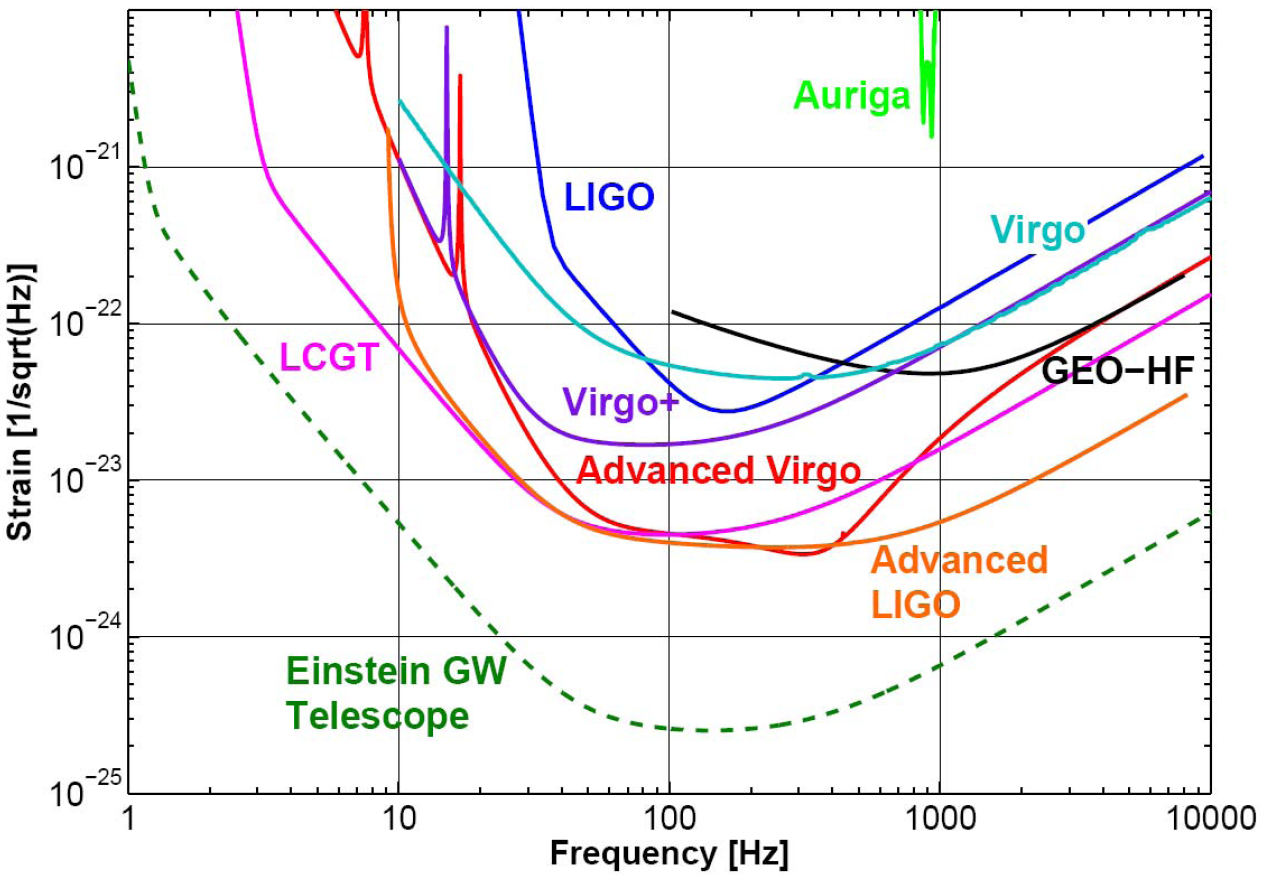
\includegraphics[width=0.6\textwidth]{Sec_Introduction/3gen_sens.png}
	\caption{Sensitivities of gravitational wave detectors from the first to the third generation.}
	\label{fig:GW_sens_evolution}
\end{wrapfigure}
The sensitivity of gravitational wave detectors improved considerably from the bar detectors to the first generation of interferometric detectors, which are currently being upgraded to the the 'advanced' generation. The corresponding sensitivites are shown in figure~\ref{fig:GW_sens_evolution}. 
In order to achieve the scientific goals stated above, the sensitivity in comparison to the second generation of gravitational wave detectors must be improved by about an order of magnitude over the entire detection frequency band ranging from 10\,Hz to about 10\,kHz. Frequent observation of low frequency sources, e.g. intermediate mass black holes, requires an extension of the detection range towards lower frequencies. \\
The initial sensitivity goal for the Einstein Telescope, estimated at the start of the Design Study, as shown in figure~\ref{fig:GW_sens_evolution}, was driven by the need to get frequent high Signal to Noise Ratio (SNR) \nomenclature[aSNR]{SNR}{Signal to Noise Ratio} events for routine gravitational wave astronomy. The high frequency sensitivity was given by the maximum power feasible, the mid frequency range was governed by thermal noises and the low frequency range by either thermal or seismic noises. The initial estimates have been refined during the design study and finally resulted in the sensitivity shown in figure~\ref{fig:ET_sens_evolution_2}.\\
\subsubsection{Size, shape and layout}
The conceptual design of a project of this financial scale (see table~\ref{Fig:TotalCostTable}) has to be based on well proven and experimentally tested techniques. The sensitivity, which the Einstein Telescope project aims for, on the other hand, needs to exploit all state of the art technologies and drive them to their physical limits. 
\begin{wrapfigure}{r}{0.4\textwidth}
%\begin{figure}{H}
	\centering
		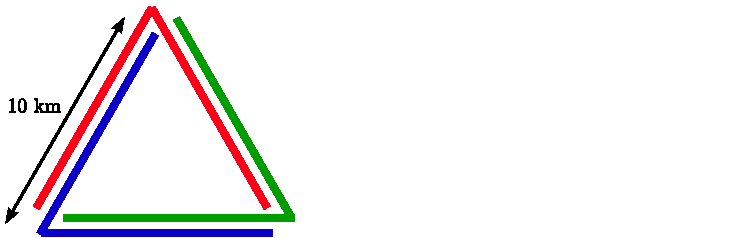
\includegraphics[width=0.3\textwidth]{Sec_Introduction/NestedDetectors.pdf}
	\caption{Three nested detectors in a triangular arrangement will form the final Einstein Telescope geometry.}
	\label{fig:NestedDetectors}
\end{wrapfigure}
This sensitivity can only be reached by significantly increasing the size of the detector beyond the size of currently available instruments (i.e.\ 3\,km for Virgo and 4\,km for LIGO) and going to an underground location where the seismic noise is lower than at the surface. Only by increasing the arm length to 10\,km the influence of unavoidable displacement noises can be lowered to a sufficiently low level.\\
In its final construction stage the Einstein Telescope will consist of three nested detectors, which will be arranged in a triangular pattern as shown in figure\,~\ref{fig:NestedDetectors}. 
In contrast to the traditional L-shaped geometry of the first and second generation of gravitational wave detectors this arrangement is equally sensitive for both polarisations of the gravitational wave. Additionally it shows a more isotropic antenna pattern compared to the L-shaped detectors, as shown in figure\,~\ref{fig:triangleAP}. The overall frequency range covered will reach from a few Hertz to about 10\,kHz.

Each individual detector in turn will comprise two interferometers, one specialised for detecting low frequency gravitational waves and the other one for the high frequency part. The sensitivity goal for each interferometer is shown in figure\,\ref{fig:ET_sensitivity}. \\
\nomenclature[gdualrec]{dual Recycling}{Using Power- and Signal-Recycling at the same time}
\nomenclature[gpowerrec]{Power Recycling}{Re-using the light reflected back to the interferometer input by placing a mirror there and resonantly enhancing the circulating light power. Has the same effect as using a more powerful laser.}
\nomenclature[gsignalrec]{Signal Recycling}{Resonantly enhancing the GW signals exiting the interferometer through the output port by placing a mirror there and resonantly enhancing the GW signals. This increases the sensitivity at the cost of the bandwidth. With a different (anti-resonant) tuning the same technique can be used for widening the bandwith at the expense of the sensitivity (RSE). SR can optimize the sensitivity for an arbitrary frequency}
\nomenclature[aRSE]{Resonant Sideband Extraction}{The same technique as SR but operated anti-resonant, i.e.\ widening and/or detunning the bandwith by reducing the reflectivity of the compound mirror formed by the inboard cavity mirror and the SR mirror.}
\nomenclature[aSR]{SR}{Signal Recycling}
\nomenclature[aPR]{PR}{Power Recycling}
Each individual interferometer has a classical dual recycled Michelson topology with arm cavities. This is a mature technique, well tested in laboratory experiments, and currently being set up for the second generation detectors LIGO and Virgo. More elaborate topologies like Sagnac interferometers or optical bars using Quantum non-Demolition (QND) techniques do not promise significant advantages and have not yet reached the level of maturity required for a project of this scale.\\
\nomenclature[aQND]{QND}{Quantum-Non-Demolition}
\newcommand{\glossQND}{\cite{QNDRevModPhys.68.755} describes QND techniques as follows:
"`Several high-precision physics experiments are approaching a level of sensitivity at which the intrinsic
quantum nature of the experimental apparatus is the dominant source of fluctuations limiting the
sensitivity of the measurements. This quantum limit is embodied by the Heisenberg uncertainty
principle, which prohibits arbitrarily precise simultaneous measurements of two conjugate observables
of a system but allows one-time measurements of a single observable with any precision. The
dynamical evolution of a system immediately following a measurement limits the class of observables
that may be measured repeatedly with arbitrary precision, with the influence of the measurement
apparatus on the system being confined strictly to the conjugate observables. Observables having this
feature, and the corresponding measurements performed on them, have been named quantum
nondemolition or back-action evasion observables."'}
\nomenclature[gQND]{QND}{\protect\glossQND}

\subsubsection{Quantum Noise} 
In order to achieve a sufficient sensitivity at high frequencies the light power in the arms of the high frequency interferometer needs to be increased to the Megawatt range. Thermal noise considerations on the other hand require cryogenic optics to reach the sensitivity goal at low frequencies. 

\begin{wrapfigure}{r}{0.6\textwidth}
%\begin{figure}{H}
	\centering
		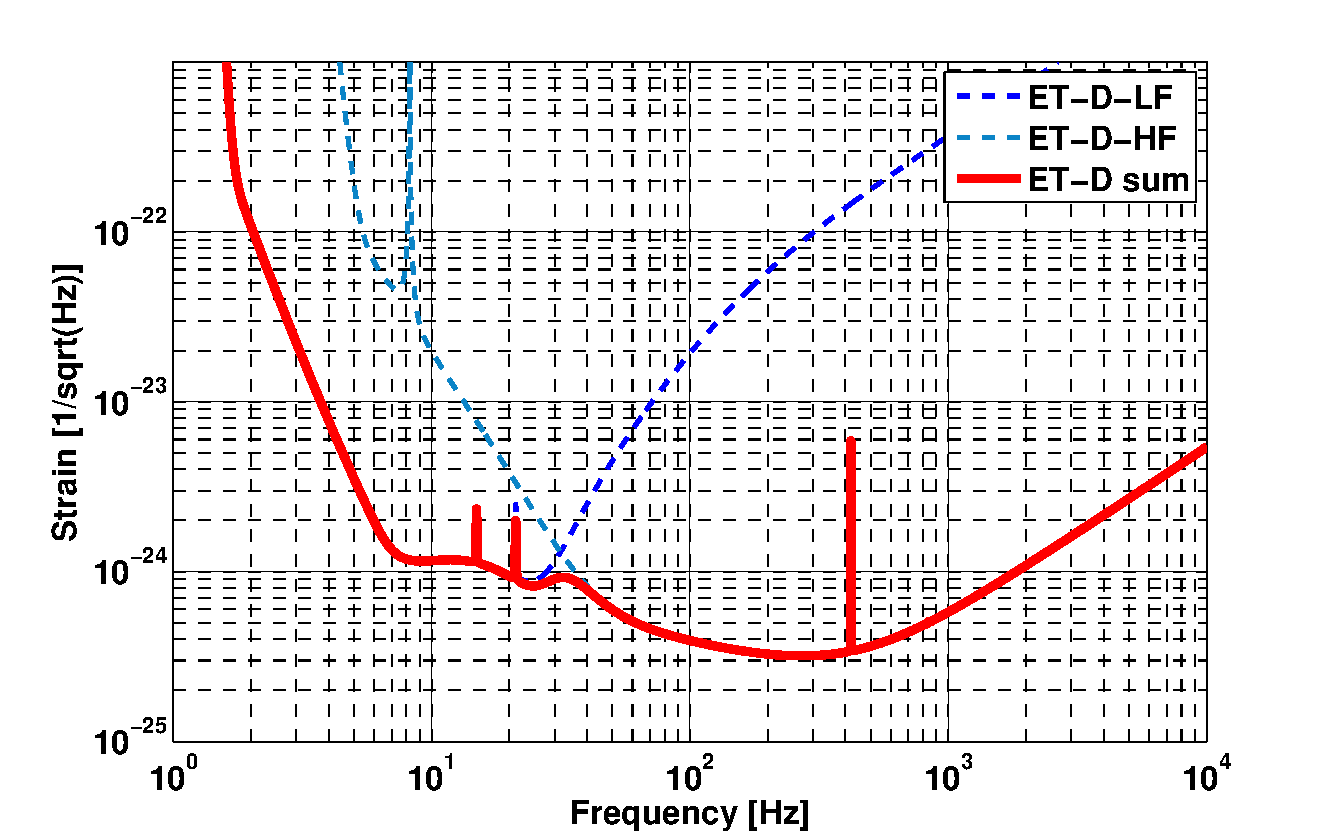
\includegraphics[width=0.6\textwidth]{Sec_Introduction/ET_D_spectrum.pdf}
	\caption{Sensitivity of the Einstein Telescope in the `Xylophone' configuration. The sensitivity of the low frequency cryogenic interferometer is shown in the dashed dark blue curve and the one of the high frequency room temperature one in a dashed blue-green tone. The sum of both is given by the solid bright red curve.}
	\label{fig:ET_sensitivity}
\end{wrapfigure}

Operating cryogenic optics at a level of several Megawatt of light power presents a serious technological challenge which is extremely hard to master. Even for the best mirrors that state of the art of coating technology can produce, the residual absorption of only about one ppm leads to an absorbed power of several Watts at a circulating light power level in the Megawatt range. The resulting thickness of the suspension fibres, which would be needed to remove the heat, would spoil the performance of the ultra low loss suspension. The Einstein Telescope will therefore be realised in what we call a 'Xylophone' arrangement, where each single detector is split into two interferometers as shown in figure~\ref{fig:ET_sensitivity}. The one dedicated for detecting high frequency gravitational waves in the range from about 30 Hz to 10 kHz will be operated at room temperature, use fused silica optics with a diameter of about 60\,cm and a mass of about 200 kg each, have a light power of about 3 MW in the interferometer arms, and run with broadband tuned signal recycling. The cryogenic, low frequency one, operated at a temperature of 10\,k and aimed at the frequency range from 1.5 Hz to 30 Hz, will use detuned signal recycling, 18 kW in the interferometer arms, and silicon mirrors with a diameter of about 40\,cm and a mass of about 200 kg. The cryogenic optics will either be made of sapphire or, more likely, of silicon. The dimensions will partly be determined by the maximum availabe bulk material size and otherwise be comparable to the room temperature ones. A summary of the main parameters for the high and low temperature interferometers is given in table~\ref{tab:summary14}.\\
 The high mirror mass will not only keep radiation pressure effects low but also allow larger sized beams spots on the mirror surfaces for lowering thermal noise effects. This split detector arrangement also offers an elegant solution for the challenge that radiation pressure noise and shot noise scale conversely with light power and cannot individually be optimised in a single interferometer. In an interferometer using classical states of light the the so-called Standard Quantum Limit (SQL) \nomenclature[aSQL]{SQL}{Standard Quantum Limit} determines the lower limit for the quantum noise. For each frequency it is another individual and optimal compromise between shot noise and radiation pressure noise, meaning that in a single interferometer the SQL cannot be reached for all frequencies simultaneously. 
 
\begin{wrapfigure}{r}{0.35\textwidth}
%\begin{figure}{H}
	\centering
		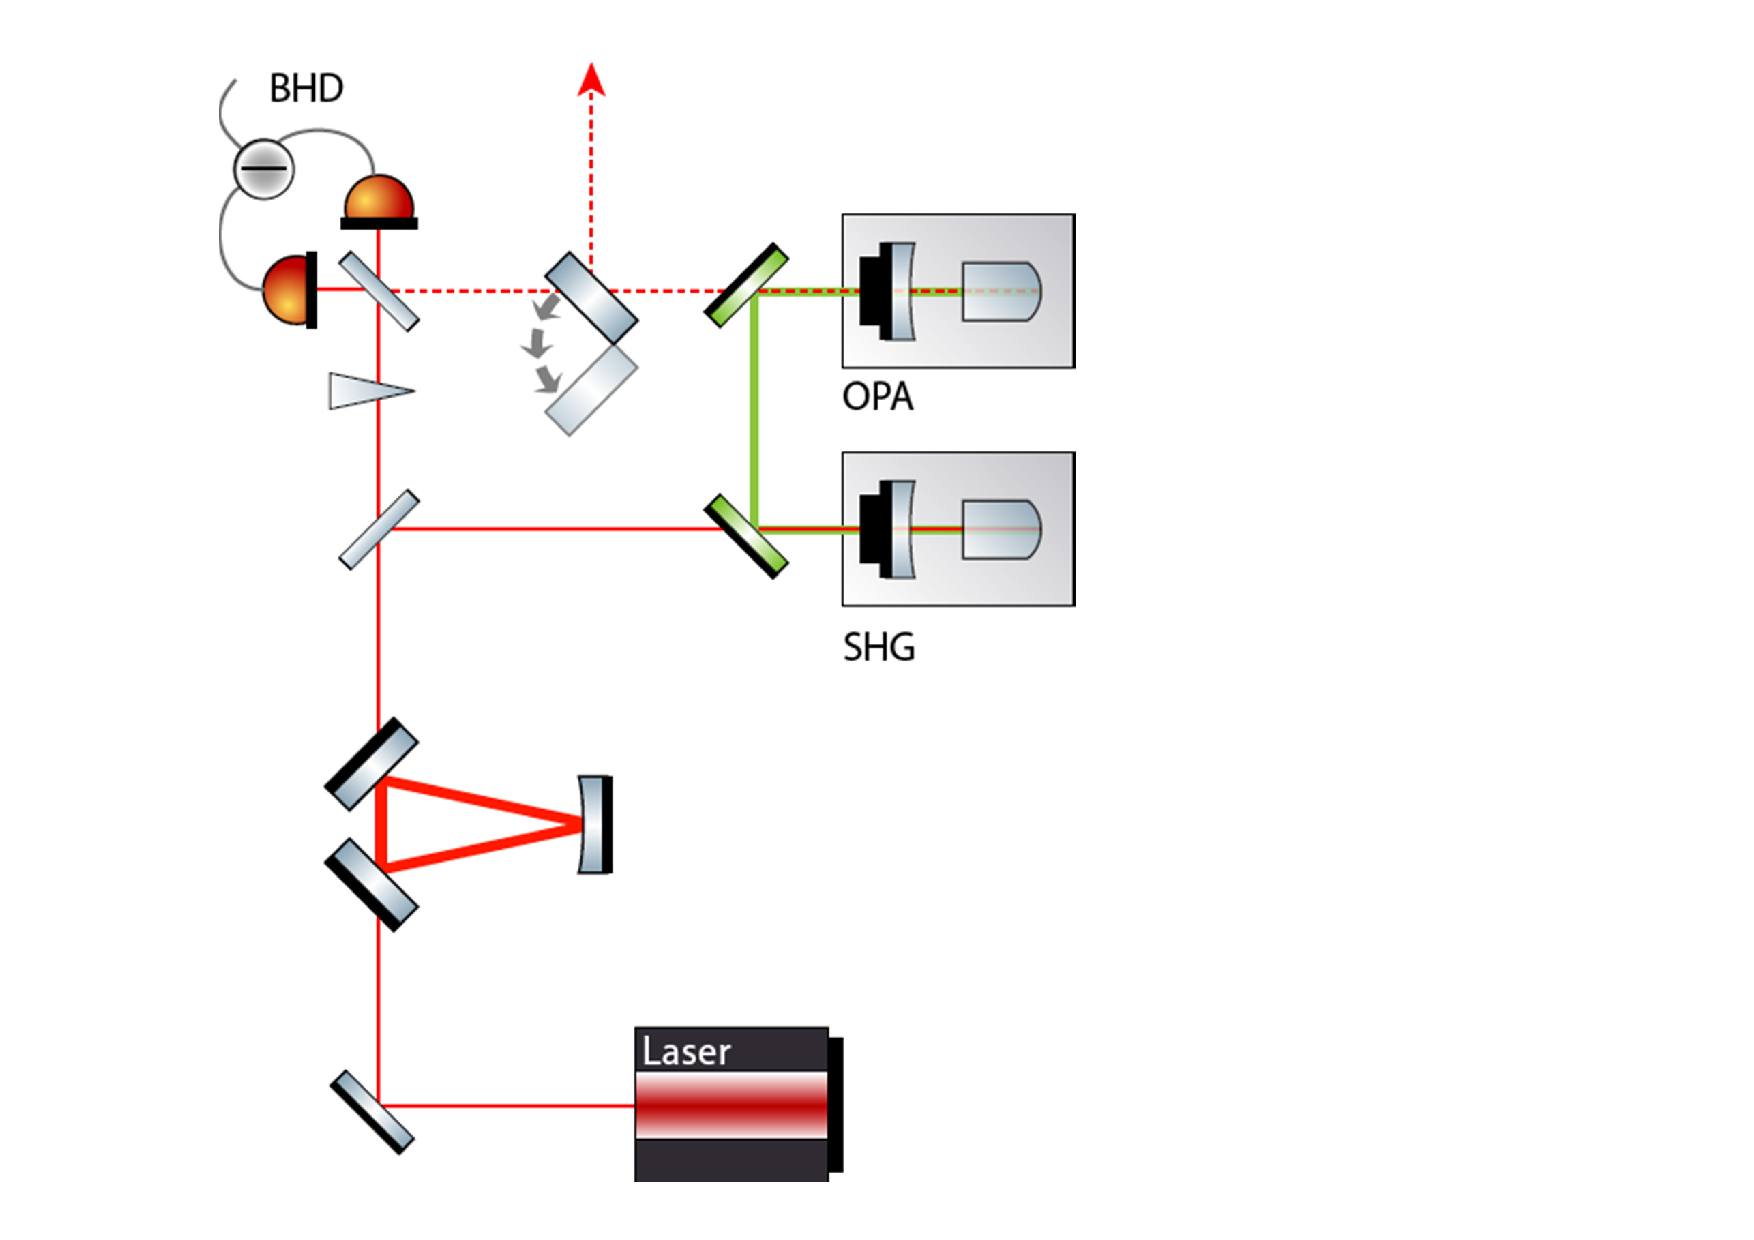
\includegraphics[width=0.35\textwidth]{Sec_Introduction/SqzGenIntro.pdf}
	\caption{Scheme for generating squeezed light. For details see section~\ref{subsec:SQZforGWD}}
	\label{fig:SqzGenIntro}
\end{wrapfigure} 

It can only be overcome if nonclassical light with correlations between the phase and the amplitude quadrature is used, so-called squeezed light. In the shot noise dominated frequency range squeezed light, which shows lower phase fluctuations at the cost of the amplitude fluctuations in comparison to classical laser light in the interferometer arms, is used. In the low frequency, radiation pressure dominated range the fluctuations need to be lowered in the amplitude quadrature. This goal can be achieved by reflecting squeezed light off a filter cavity (see figure \ref{Fig:opt_lay_over}). The squeezing level and with it the sensitivity improvement that can be reached, depends on the optical losses in the squeezer, the filtering optics, the interferometer, and all optical devices on the way to the photodetector including the photo detector efficiency itself. Squeezing levels over the full observation band width of up to 10\,dB and stable long-term operation and best squeezing values of 13\,dB have been demonstrated. The usage of squeezed light is currently tested in the existing gravitational wave detectors and is foreseen as an add-on to the second generation. For the Einstein Telescope we assume 15\,dB initial squeezing level at the squeezing source and an effective squeezing level of 10\,dB to be available (equivalent in shot noise reduction to a laser power increase of a factor of 10). Optical losses easily add vacuum fluctuations \nomenclature[gVACFLUC]{vacuum fluctuations}{fluctuations that result from the quantum nature of an electro magnetic field even at the lowest possible energy level (zero mean energy = vacuum)} to the squeezed quadrature and hence reconvert squeezed light into classical light. It will therefore be essential to keep the optical losses as low as possible. Optical losses of 75\,ppm per round-trip are currently achievable with state of the art techniques and are used as a conservative estimate for the filter cavities.

\subsubsection{Thermal Noise}
\begin{wrapfigure}{r}{0.65\textwidth}
%\begin{figure}{H}
	\centering
		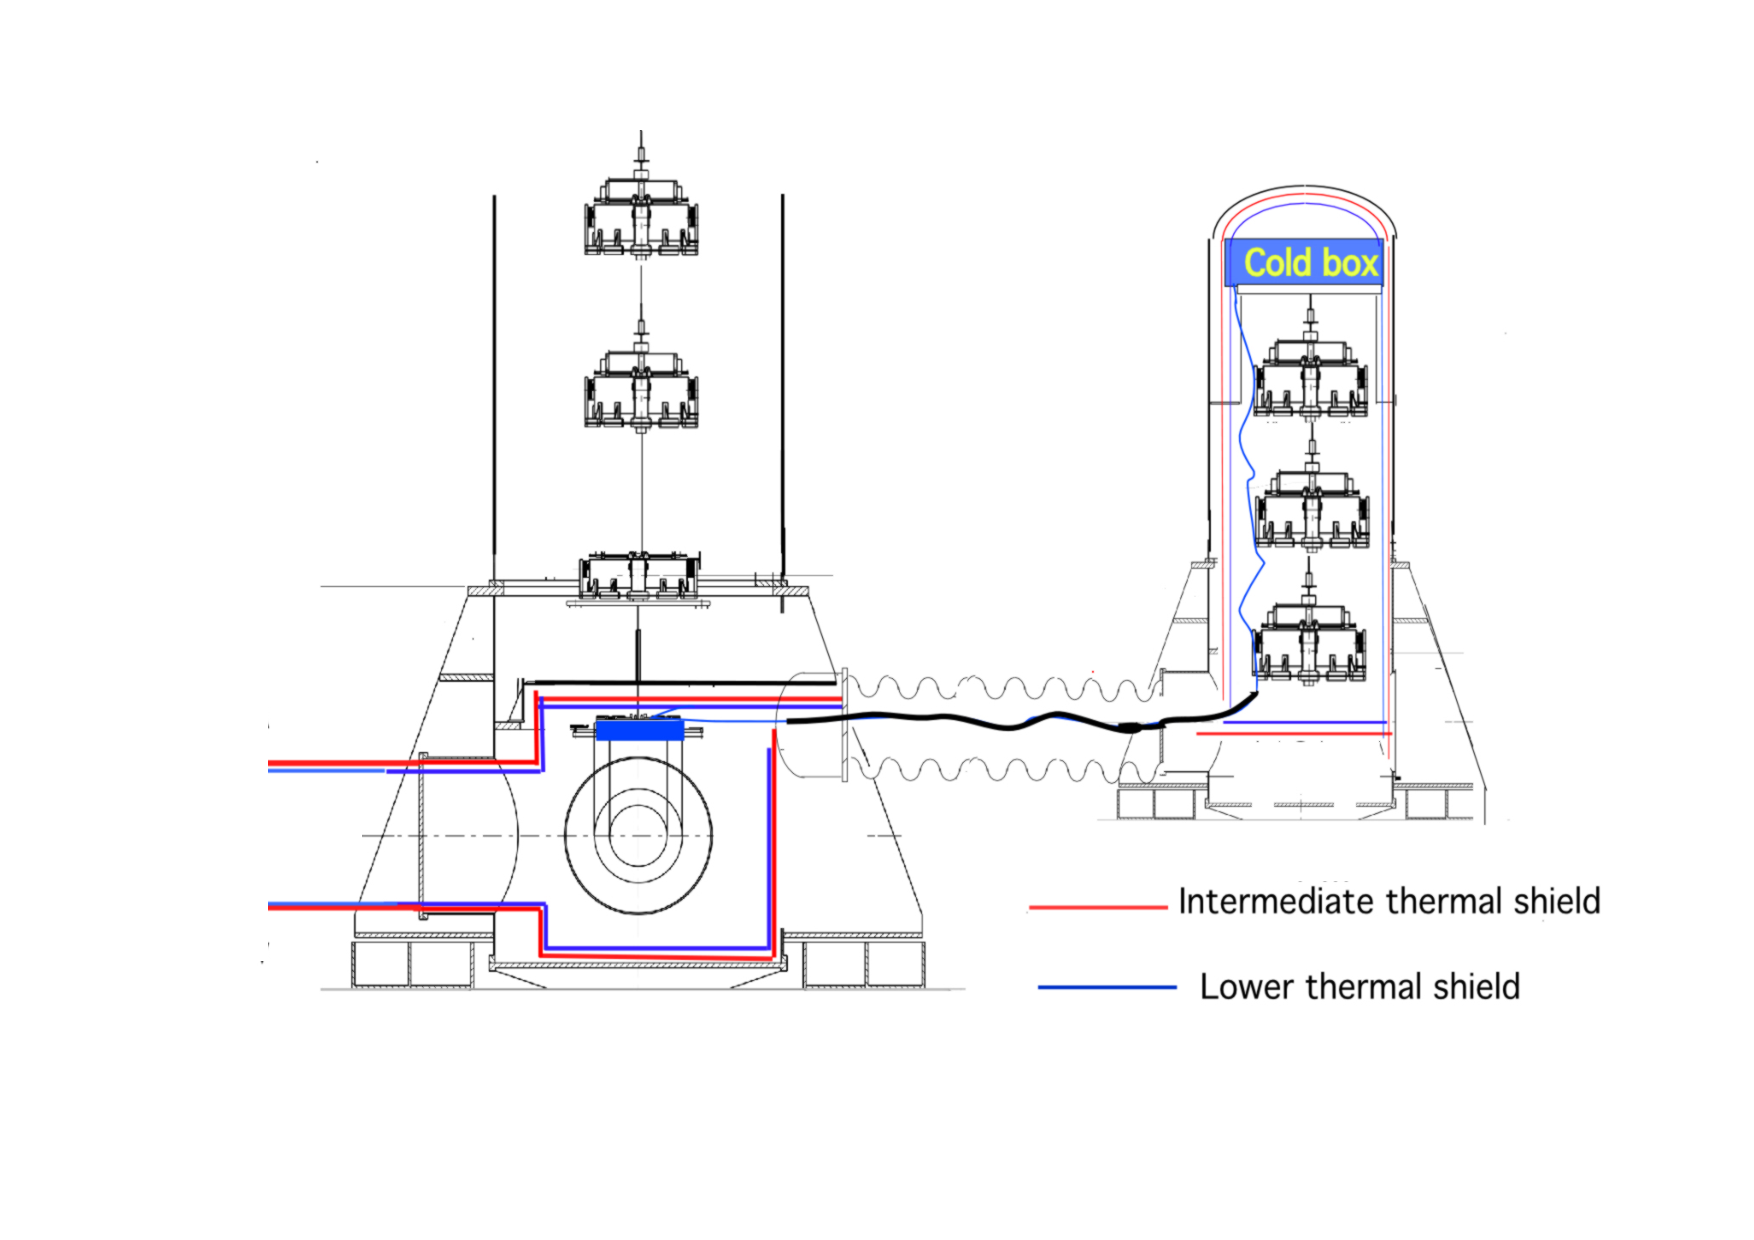
\includegraphics[width=0.65\textwidth]{./Sec_SiteInfra/Figures/ET_main-cryostat.pdf}
	\caption{Scheme for cooling the mirrors. For details see section~\ref{cryo}}
\end{wrapfigure} 

Reaching the sensitivity goal at low frequencies requires a significant reduction of thermal noises compared to the first and second generation of gravitational wave detectors, which can be achieved by operating the mirrors at cryogenic temperatures as low as 10\,K.  

Cryogenic operation is also foreseen for the final stage of the planned Japanese gravitational wave detector LCGT \nomenclature[aLCGT]{LCGT}{Large Scale Cryogenic Gravitational Wave Telescope. A second generation gravitational wave detector built in Japan}. At these low temperatures fused silica has got a low mechanical quality factor and becomes unusable. Silicon and Sapphire show excellent low temperature behaviour (see section~\ref{sec:app}) and are good candidates for cryogenic gravitational wave detectors. The availability in large quantities and good purity through the semiconductor industry makes silicon a promising candidate for the Einstein Telescope cryogenic optics. Some quantities such as the temperature dependence of the refractive index at low temperatures and the residual optical absorption in ultrapure silicon, although assumed to be good enough for the Einstein Telescope, are currently not known and need to be investigated in R\&D activities.

Removing the heat generated by laser light being absorbed at the mirror surfaces without introducing excess vibration levels poses another technical challenge. As thermal radiation does not provide sufficient coupling at cryogenic temperatures this heat removal has to be done by thermal conduction of the suspension fibres. The resulting requirement for the thickness of the silicon suspension fibres needs to be balanced against good seismic isolation properties of thin fibres. The vibration level of cryo coolers, which could be placed close to the optics, threatens the low frequency sensitivity (see section~\ref{sec:cryocoolers}). R\&D in active and passive vibration suppression is still required to sufficiently cut the remaining noise level down for use in the Einstein Telescope. Cryo fluids, like superfluid Helium~II, which are cooled down at a remote location above ground, are foreseen as a seismically more quiet alternative (see section~\ref{sec:Helium_II}). The final operating temperature for the Einstein telescope remains to be fixed in a technical design phase. The cooling capabilities foreseen so far will allow using mirror temperatures as low as 10 Kelvin.

\subsubsection{Seismic Isolation}

\begin{wrapfigure}{r}{0.4\textwidth}
%\begin{figure}{H}
	\centering
		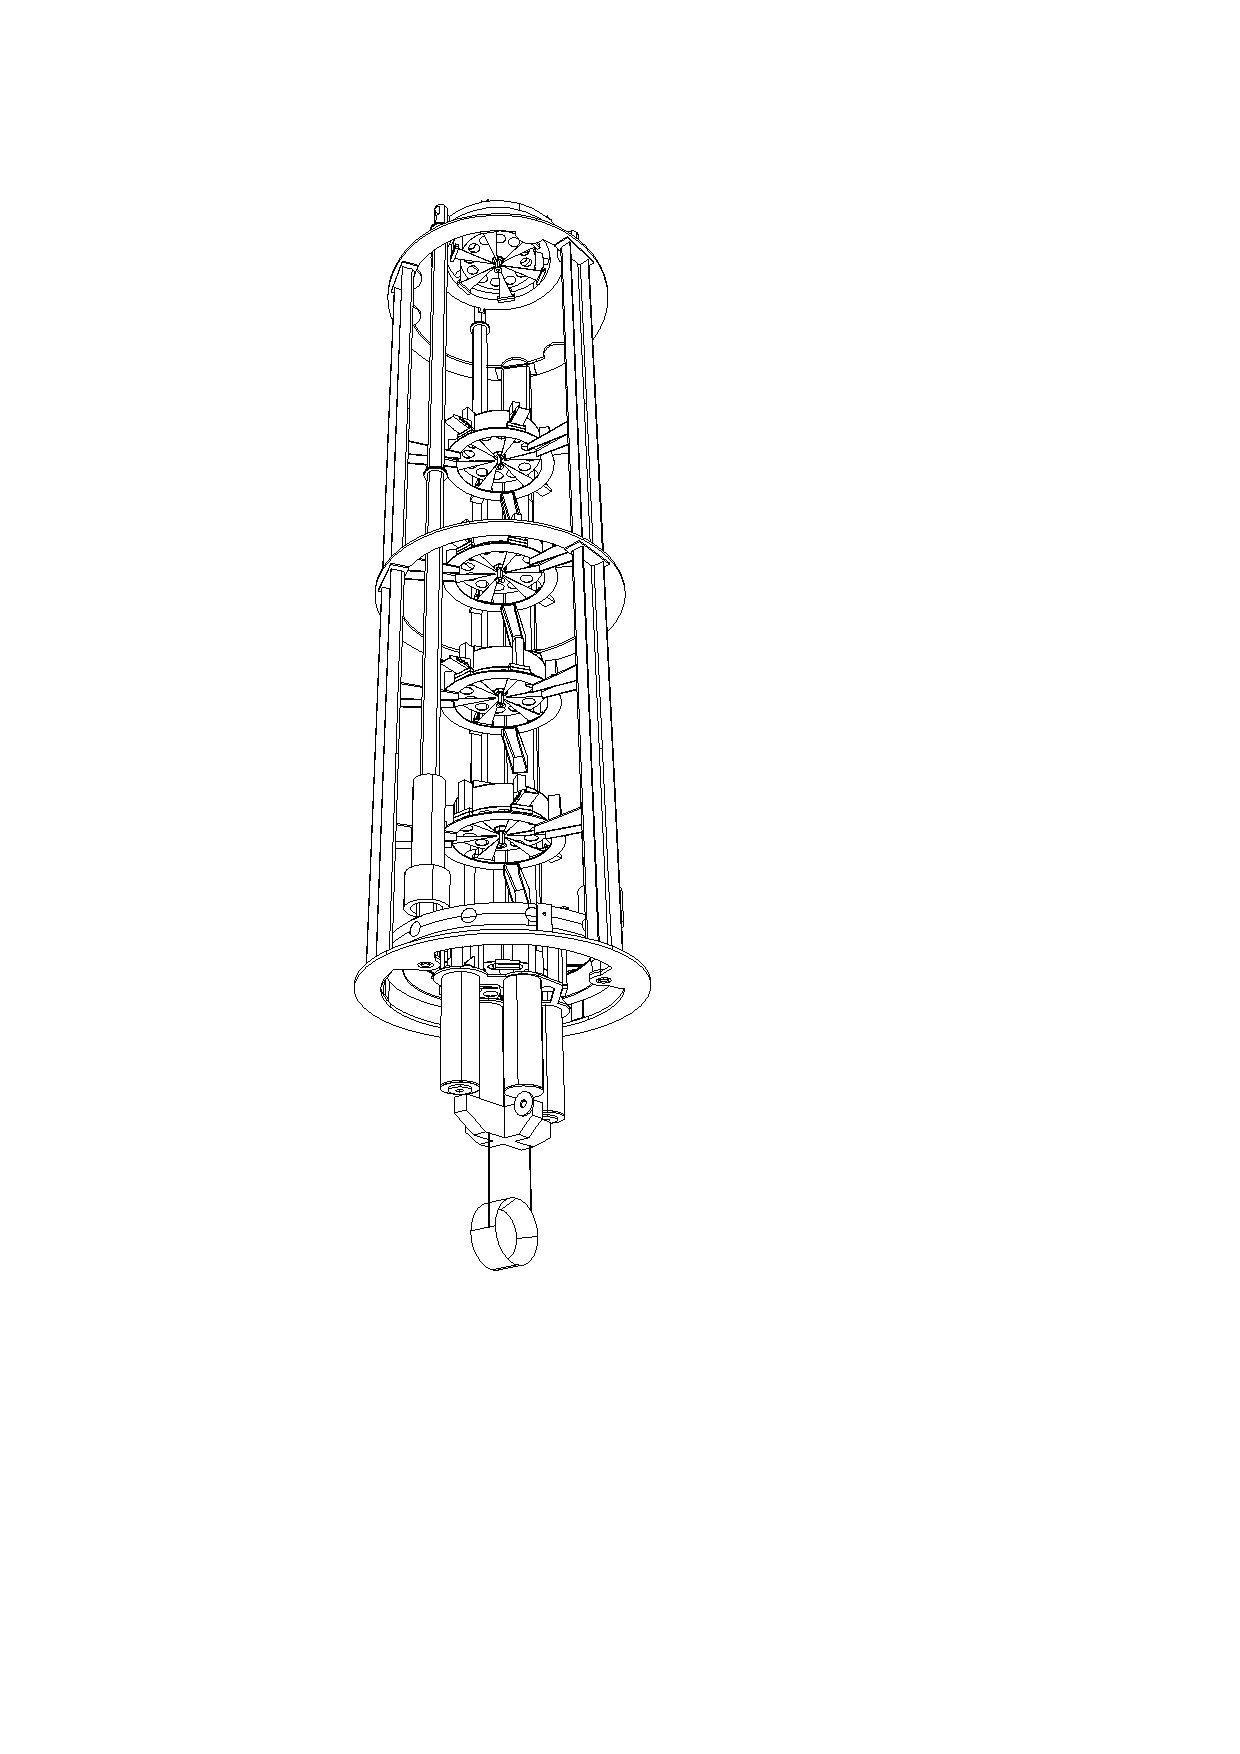
\includegraphics[width=0.18\textwidth]{./Sec_Introduction/VirgoSA.pdf}
	\caption{Schematic view of the Virgo Superattenuator. See also section~\ref{sec:suspension_systems}}
\end{wrapfigure} 

The main optics for the Einstein telescope need to be very well isolated against seimic ground motion. For the second generation of gravitational wave detectors both, active and passive isolation strategies are being pursued. In the advanced LIGO detectors a two stage system actively isolates a platform from ground motion, from which the main optics are suspended by quadruple pendulums. The passive strategy employed at the Virgo detector, demonstrated an excellent performance over the full frequency range (see figure \ref{FigSusp5}) and is foreseen as the reference solution for the Einstein telescope. The horizontal isolation is achieved with a six-stage pendulum system, whereas for the vertical degree of freedom cantilever springs  are used. The pendulum suspension system itself is supported by a platform resting on an inverted pendulum, which provides additional horizontal seismic isolation (see figure~\ref{SAfig1}). All mechanical resonances of the whole structure are actively damped to avoid resonant mechanical amplification of ground motion. The overall height of the suspension system is about 17\,m, requiring correspondingly tall vacuum chambers and caverns.

\subsubsection{Newtonian gravity gradient noise}
 Newtonian gravitational interactions between the optics and the surrounding soil provide a direct coupling mechanism of ground motion to the interferometer test masses (see also section~\ref{NewtonianNoise}). As the resulting, so-called gravity gradient noise cannot be shielded from the mirrors, a location has to be found where this seismic motion is minimal and the surrounding soil as homogeneous as possible. This goal can be achieved in an underground location in a seismically quiet region. Preliminary measurements show that a depth of 100 to 200m in a remote location with low population density provides sufficiently low seismic motion. The potential of measuring the ambient seismic motion, feeding it into a gravity gradient noise model, and then subtracting the predicted effect from the interferometer output signal has been investigated. Initial results are promising, and are interesting also for the second generation of gravitational wave detectors, but investigations need to be continued in an R\&D programme (see section~\ref{subsub:AmbientNNsubtraction}).
 
 \subsubsection{Vacuum}
 The space between the mirrors in the interferometer arms has to be evacuated to very low residual partial gas pressures to keep the apparent length changes caused by fluctuations of the refractive index sufficiently low. The tolerable maximum pressure is on the order of $\rm{10^{-8}}$~Pa (see paragraph~\ref{average pressure}).
 
 Some technical parameters will remain "to be defined" in this design study document. At this stage of the conceptual design these parameters are not important and will be worked out in a future technical design phase.

\subsubsection{\label{Noisebudget}Noise budget}

\begin{wrapfigure}{r}{0.65\textwidth}
  \begin{center}
    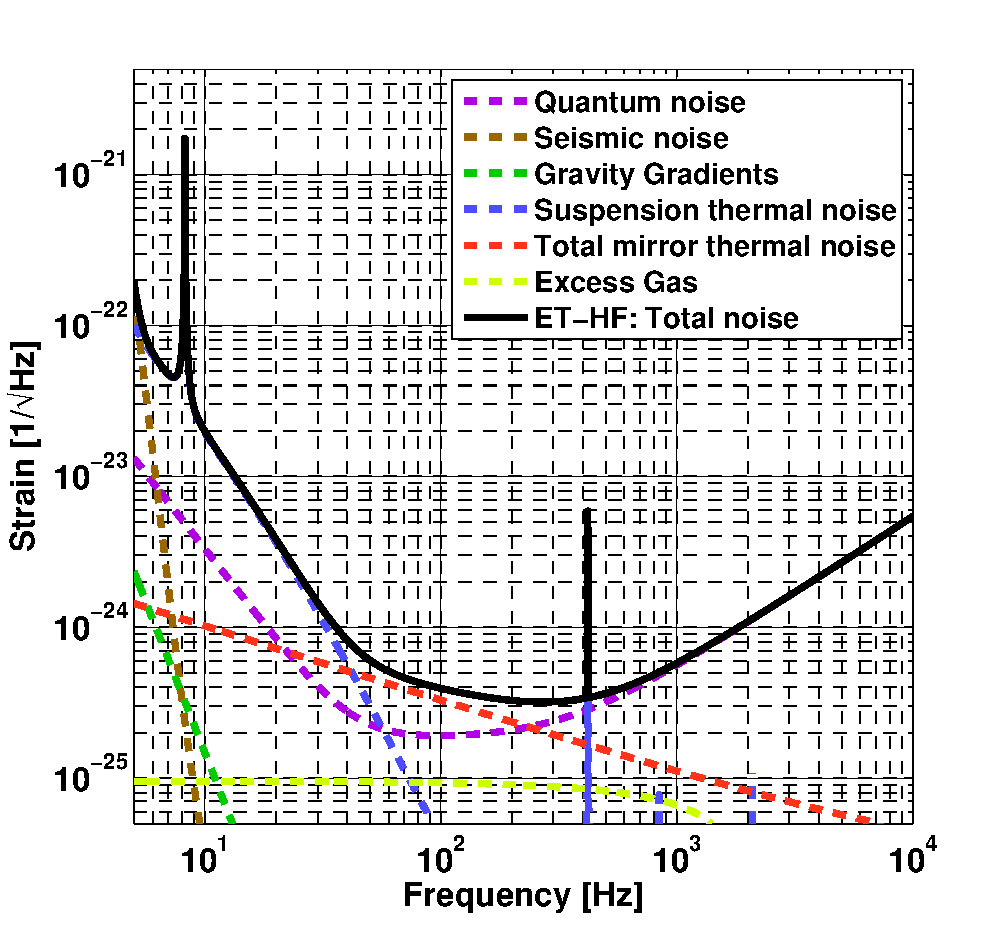
\includegraphics[width=0.45\textwidth]{Sec_Introduction/ETD_HF3.pdf}
%      \end{center}
%  \end{wrapfigure}
%  
% \begin{wrapfigure}{r}{0.6\textwidth}
%  \begin{center}
    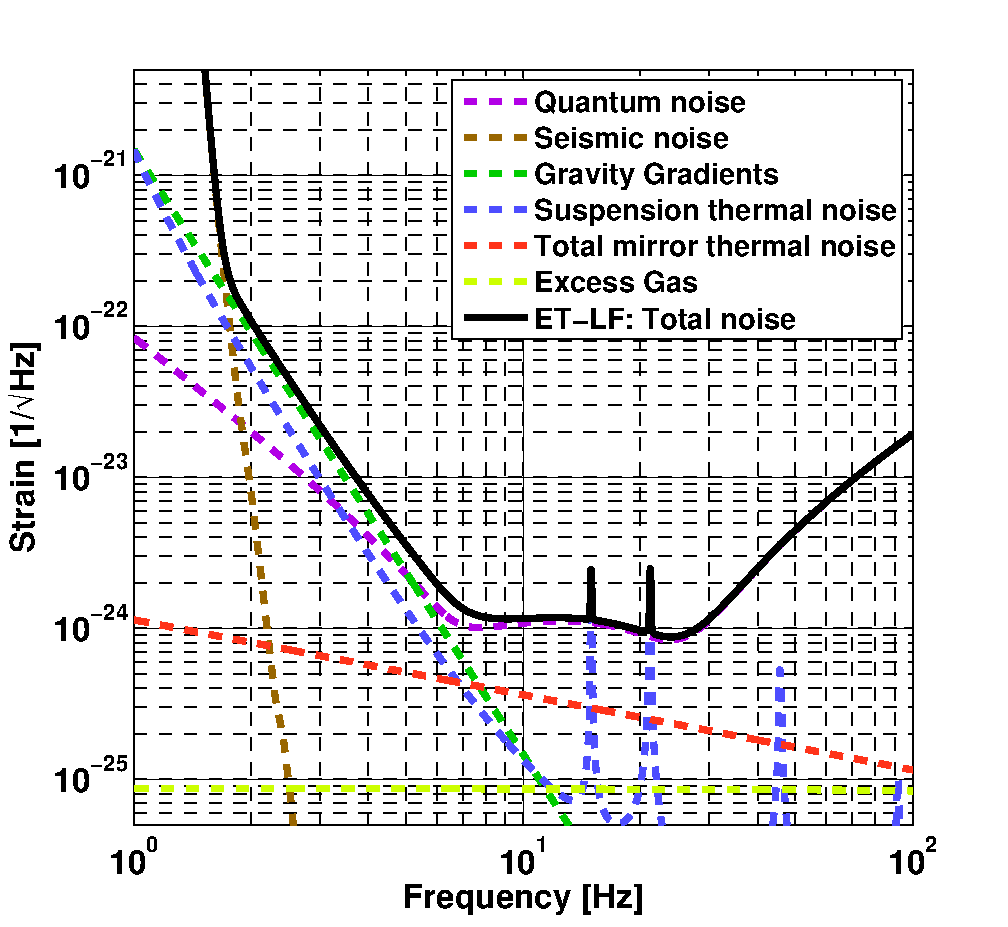
\includegraphics[width=0.45\textwidth]{Sec_Introduction/ETD_LF3.pdf}
    \caption{Noise budget for the low- and high-frequency interferometer for the parameters stated in table~\ref{tab:summary14}}
    \label{fig:noise_budget}
    \vspace{-0.7cm}
  \end{center}
\end{wrapfigure}

The Xylophone strategy, i. e. the division of each detector into a low frequency and a high frequency interferometer, allows to pursue different strategies in optimising the noise for each frequency range. The noise budget for the high frequency interferometer is shown in upper part of figure~\ref{fig:noise_budget}. 

In the frequency range from about 7~Hz to 30~Hz the sensitivity is limited by suspension thermal noise, resulting from the interferometer being operated at room temperature. At frequencies above 500 Hz the dominating noise source is photon shot noise. Between these two frequency ranges mirror thermal noise is limiting the overall sensitivity. In the noise budget for the low frequency interferometer, shown in the lower part of figure~\ref{fig:noise_budget} quantum noise is limiting the sensitivity over the entire frequency range above 7~Hz. Due to the operation at cryogenic temperatures the influence of suspension thermal noise in the frequency range above 7~Hz could be cut down to a sufficiently low level. Below 7 Hz the sensitivity is limited by comparable amounts of quantum noise, gravity gradient noise, and suspension thermal noise. Due to the good performance of the multistage pendulum suspensions the influence of seismic noise can be limited to the frequency range below 2~Hz. Investigations of new quantum non-demolition techniques in a planned R\&D program will show whether it is possible to cut down the quantum noise contributions to an even lower level in the frequency range from 7~Hz to 30~Hz.

\FloatBarrier

\subsection{Layout of the observatory}
\emph{Authors: M.Punturo, H. Lueck} \\

\begin{wrapfigure}{r}{0.6\textwidth}
\centering
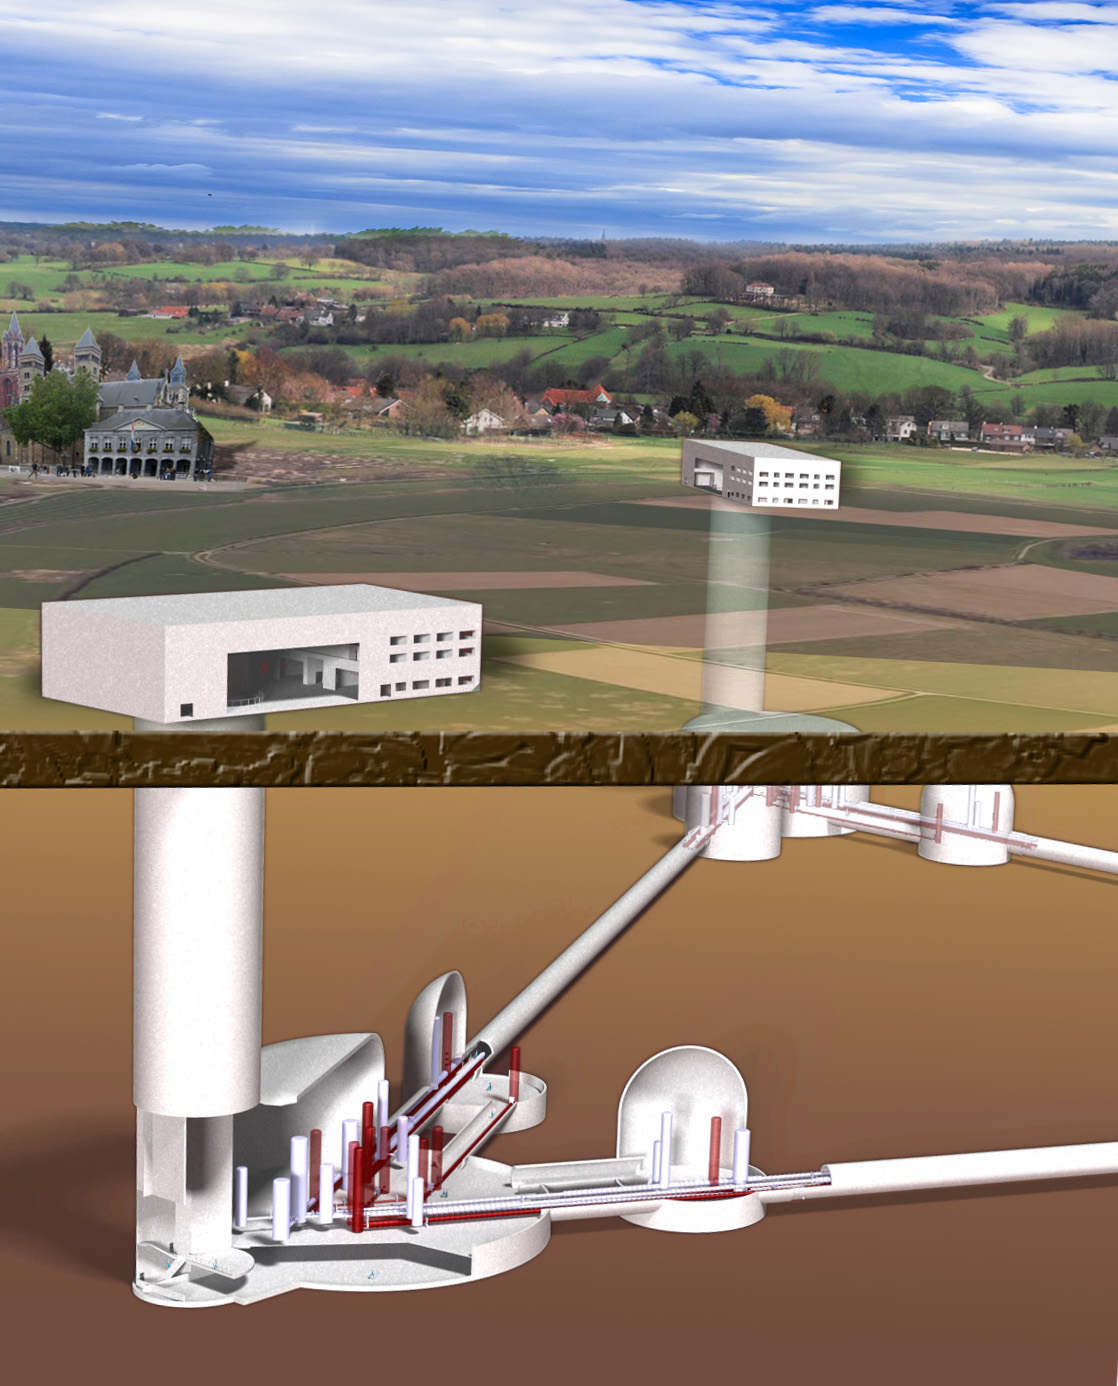
\includegraphics[width=0.6\textwidth]{Sec_Introduction/ArtisticViewBuildings.jpg}
\caption{Artistic view of the arrangement of buildings, access shafts and underground caverns.}
\label{Fig:Buildings}
\end{wrapfigure} 

As a consequence of the extremely demanding seismic requirements the Einstein Telescope will be located underground at a depth of about 100 m to 200 m and will, in the complete configuration, consist of three nested detectors, each in turn composed of two interferometers. Selecting the geometry of an equi-lateral triangle, where each side of the triangle is simultaneously used by two detector arms, optimises the usage of the tunnels and allows to determine the polarisation of the gravitational wave. The topology of each interferometer will be the dual recycled Michelson layout with Fabry-Perot arm cavities. An artists impression of the Einstein Telescope is shown in figure~\ref{fig:ET_artists_view}. \\
Underground seismic measurements at eight different European locations have been performed within this design study and additional measurements from external sources have also been evaluated. Satisfactory seismic performance has been found in several locations. 

For the final site selection long-term seismic noise measurements including seasonal effects like variable wind speeds and ocean wave height need to be made and other nonscientific factors of influence (e.g. political, financial, interest of local parties, vicinity to research institutions etc.) have to be included in the decision process.

The sensitivity curve shown in figure~\ref{fig:ET_sensitivity} gives the sensitivity for a single detector with 10\,km arm length and an angle of $90\,^{\circ}$ between the arms. This is done for better comparison with the existing detectors and their `advanced' versions. ET will in fact have three 10\,km detectors and the angles between the arms will be $60\,^{\circ}$. The resulting sensitivity in comparison with a single $90\,^{\circ}$ detector depends on the source looked at, as the angular antenna pattern (see figure \ref{fig:triangleAP}) and the polarization dependence (independent in the triangular case) influence the signal strength differently for different detector layouts. On average the sensitivity of the triple $60\,^{\circ}$ detector is slightly better than a single $90\,^{\circ}$ one.

\newpage 

\begin{wrapfigure}{r}{0.6\textwidth}
	\centering
		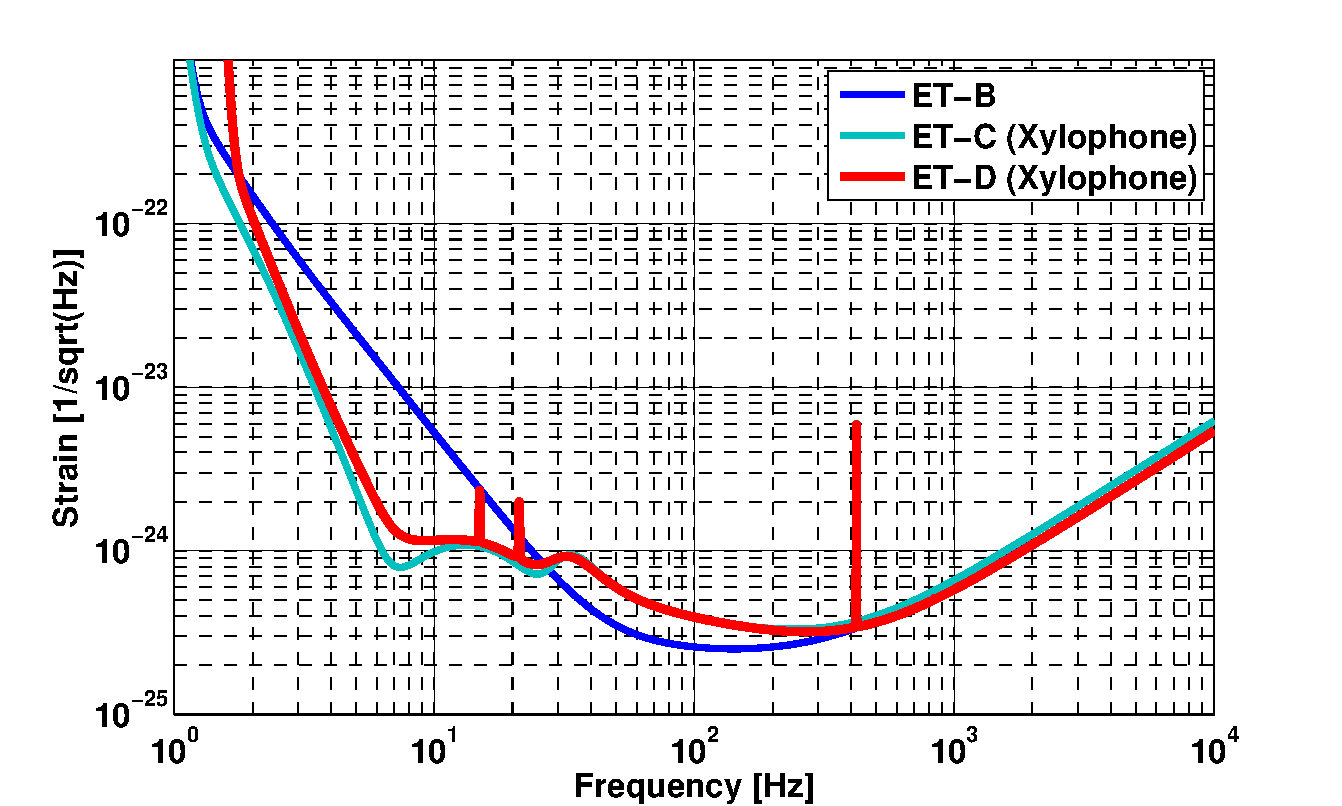
\includegraphics[width=0.6\textwidth]{Sec_Introduction/all_sens3.pdf}
	\caption{Sensitivity curves for ET used in this document. For details see text.}
	\label{fig:ET_sens_evolution_2}
\end{wrapfigure}

As the understanding of the achievable sensitivity of the Einstein Telescope evolved throughout the Design Study, different sensitivity curves are used in this document, named from ET-B to ET-D (see figure~\ref{fig:ET_sens_evolution_2}). The very first, preliminary sensitivity curve ET-A was a very rough, early estimate based on crude, obsolete estimates and will hence not be used in  his document. ET-B is the sensitivity curve where each detector is built from a single interferometer, where the high power needed to achieve good high frequency performace compromises the low frequency performance. The next evolutionary step is the sensitivity curve ET-C, where each detector is split into two interferometers, each dedicated to a distinct frequency range (the Xylophone configuration). The latest sensitivity curve is given by ET-D, where imperfections like optical losses in cavities are included in the computations. As the later sensitivity curves only became available during the Design Study, some of the subsection results are still based on earlier versions, which will be indicated by the sensitivity curve acronym.

\begin{wrapfigure}{r}{0.7\textwidth}
	\centering
		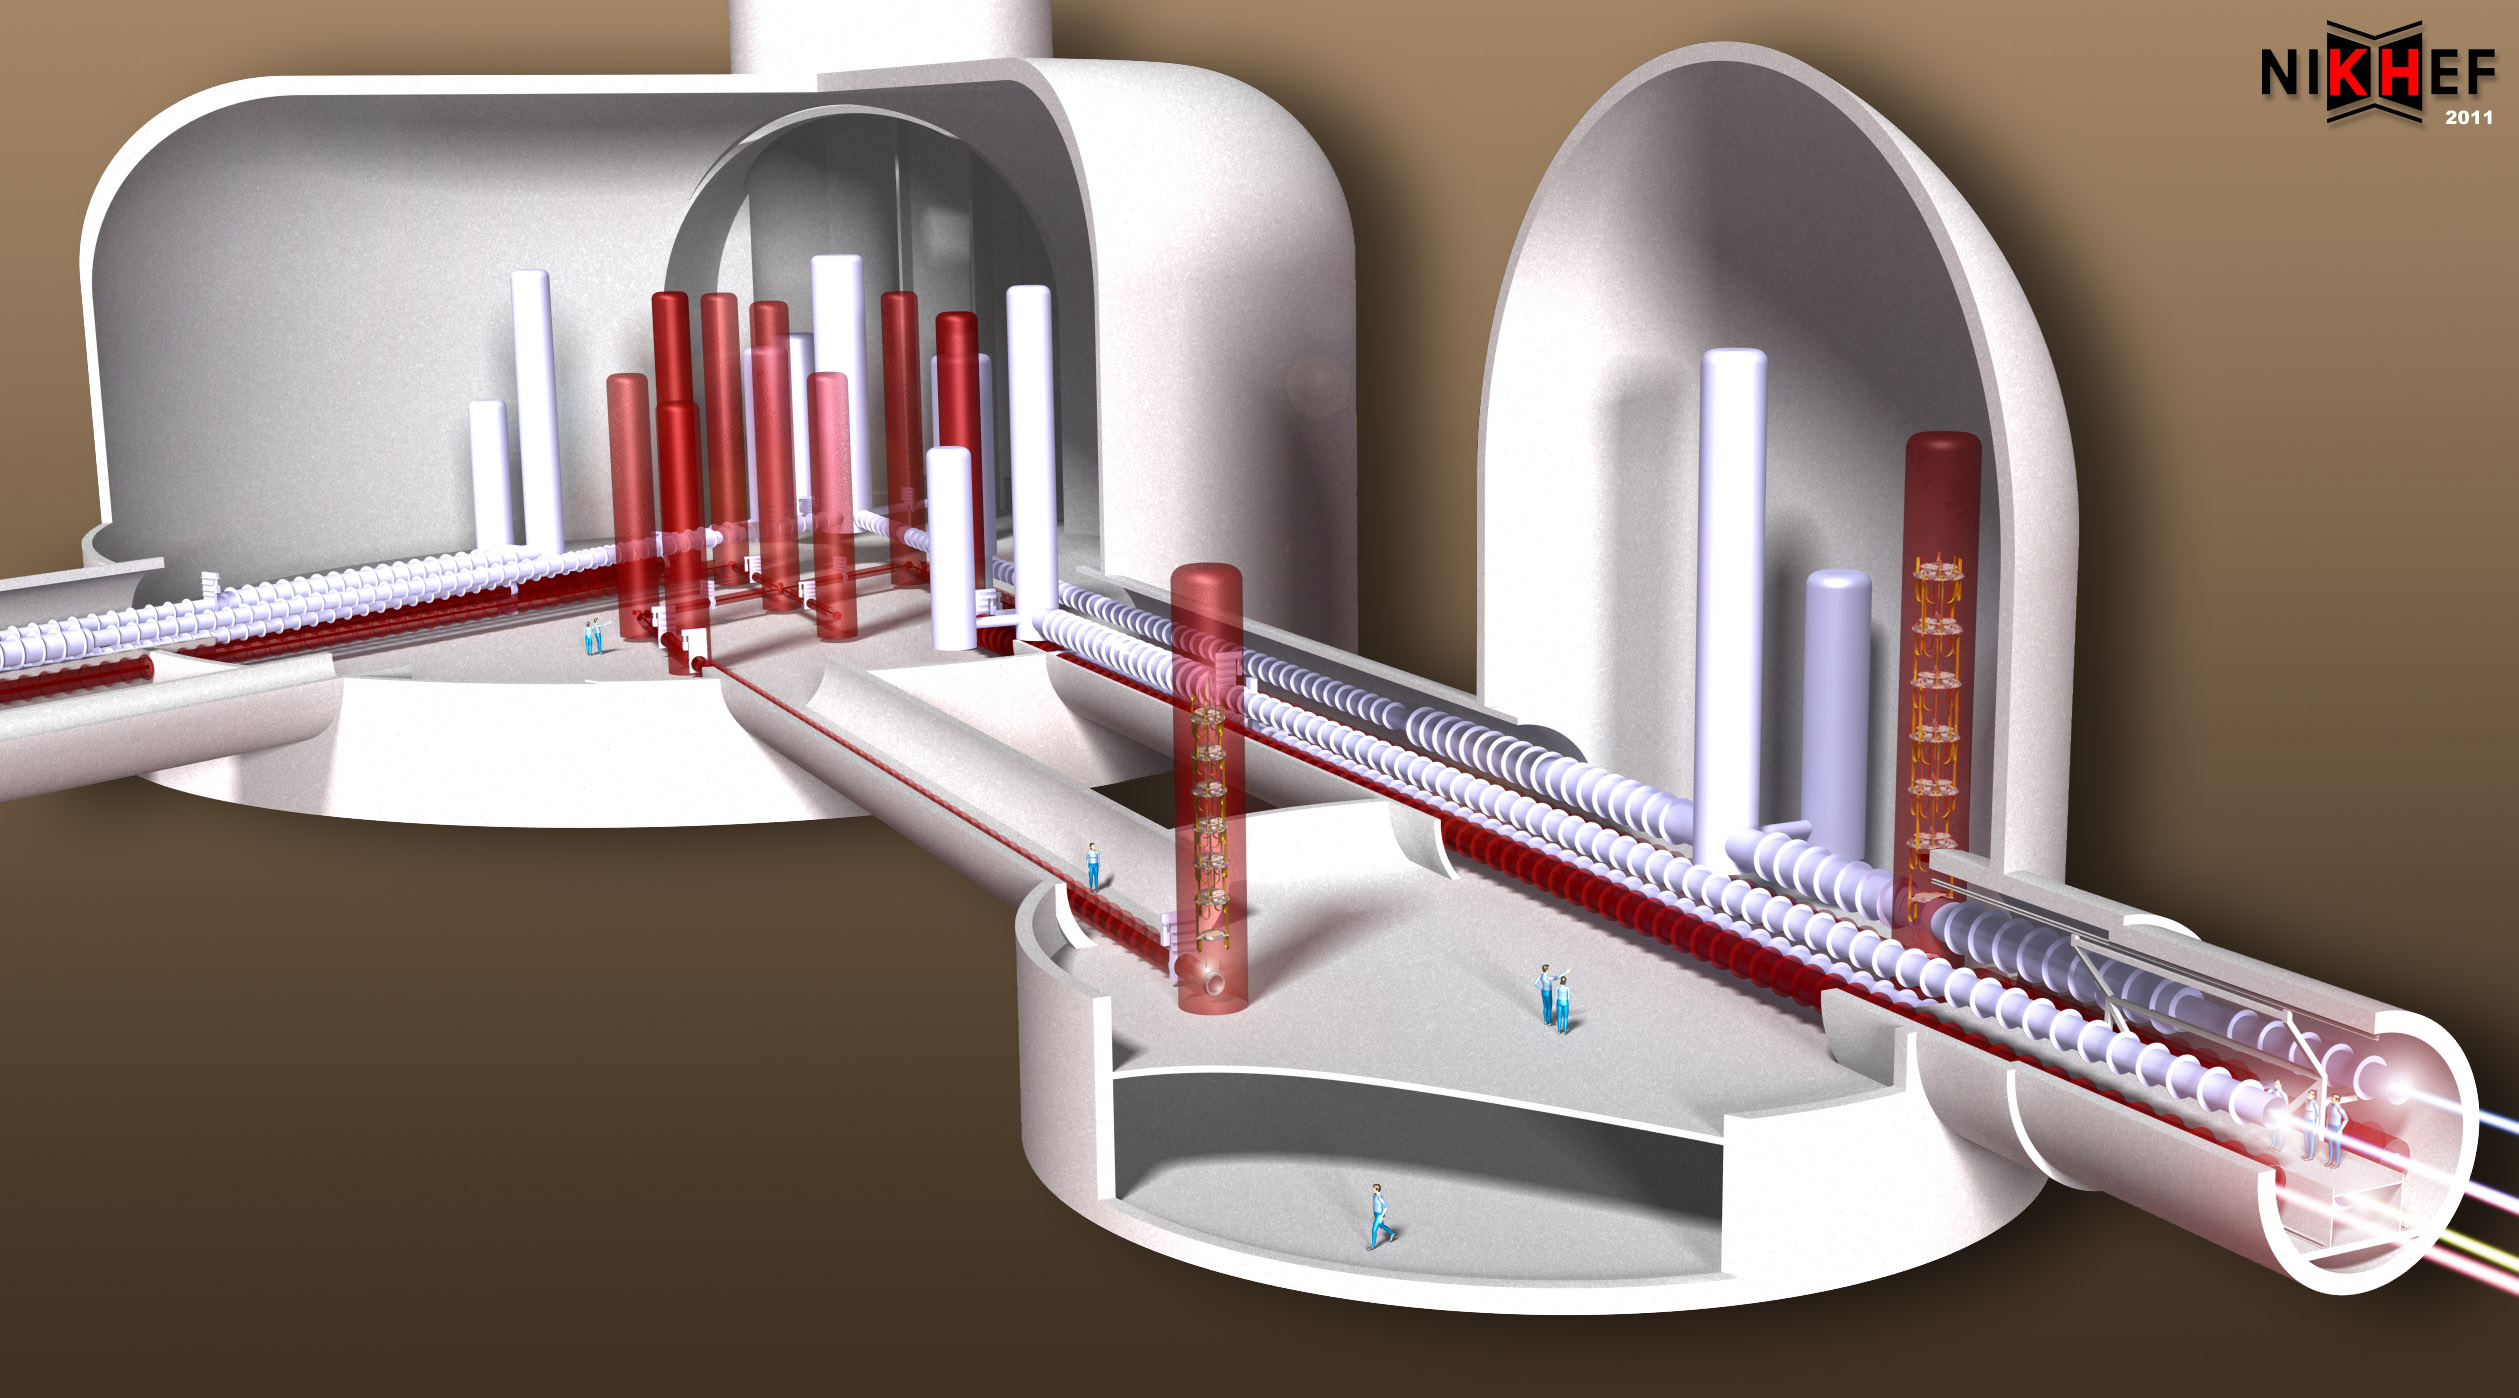
\includegraphics[width=0.7\textwidth]{Sec_SiteInfra/Figures/ArtisticView1.jpg}
	\caption{Artist impression of the underground arrangement of tunnels and caverns. For details see sections~\ref{sec:infraref} and \ref{sec:infrareal}}
	\label{fig:Artisticview1}
\end{wrapfigure}

For the desired sensitivity an overall side length of the triangle of about 10\,km is required. More specifically in this document we assume 10\,km for the arm cavity length as depicted in figure~\ref{fig:infra1} and figure \ref{Fig:Simple_ETv1} and additional 300\,m of tunnel length for telescopes for mode matching the large beam size from the interferometer arms to smaller beams in the beam splitter area. This gives a total triangle side length of 10.6\,km and an overall tunnel length for the Einstein Telescope Observatory of 31.8\,km. This length of 300 m from the "vertex station" to the "satellite station" is also used for the filter cavities for the high frequency interferometer housed in a separate tunnel, which simultaneously serves as a safety escape route from the "satellite caverns".  The main 10\,km tunnels connecting two satellite stations (see section \ref{subsec:tunnels}) will have an inner diameter of 5.5\,m, which will locally be increased to 6 .0\,m, where ever the insulation for cryogenic operation requires more space. The caverns, three vertex caverns and six satellite caverns, will house the vacuum vessels and have to be about 25\,m high (see section \ref{sec:caverns}). Access to the underground detectors is foreseen via vertical shafts (see figure \ref{fig:infra}). It remains to be explored in a technical design phase after site selection whether horizontal access is favourable. This option may for example be advantageous if the Observatory is built inside a mountain. The ET infrastructure will house the observatory for many decades, during which the interferometers will receive upgrades as technology advances. Some of these changes may result in the necessity to change mirror positions and with it vacuum tank positions as we now see in the upgrades from the 'initial' to the 'advanced' generation of gravitational wave detectors. Hence we plan to build large caverns where the tanks can be placed at arbitrary positions, instead of building an inflexible system of short tunnels connecting narrow but tall caverns housing a single vacuum tank each.  

Above ground, at the entrance to the vertical axis shafts, facilities housing workshops, offices, apartments, technical facilities providing pyogenic fluids, air conditioning and venting, emergency electricity generators, etc are
cavitiy length 10km, overall tunnel length estimated to 10.6 for 300m cavities and telescopes between inboard cavern and vertex. Tunnel diameter, escape routes used for filter cavities, vertical vs. horizontal access, cavern height, 
stress fact that it is meant to last decades.
Above ground building that houses workshops, offices, appartments, cryo facilities, air conditioning and venting facilities, emergency electricity generator, 
\FloatBarrier
\subsection{Observatory timeline}
\emph{Authors: M.Punturo, H. Lueck} \\
The realization of the ET observatory will be the final step of a long path and the initial act of a new scientific adventure. Several steps have been necessary (see Sec.~\ref{TimelineSubSection}) to allow the realization of this conceptual design study document  and few other important achievements are needed to reach the readiness condition for the observatory realization. The design of the new detector must evolve from the current conceptual phase to the technical design phase, successful R\&D activities must confirm the feasibility of the solutions proposed in this document, but, first of all, it is crucial that advanced detectors confirm the effectiveness of their new technologies and that a gravitational wave signal is detected in these interferometers. The detection of gravitational waves is regarded as a prerequisite for the start of construction of the Einstein Telescope.
For this reason the excavation of the ET site cannot start before 2017 and hence 2018 is here taken as the initial time ($t_0$) for the ET observatory realization. ET being an observatory that will be \emph{on air} for decades, the priority in the construction will be attributed to the site and infrastructures realization, selecting a modular philosophy for the detectors that will allow to implement the different interferometers composing each detector with a schedule stretched in time. In this way, after about 6 years of construction, installation and commissioning, the first detector of the ET observatory could be operative at the end of the first half of the next decade.
\FloatBarrier
\subsection{Observatory costs}
\emph{Authors: M.Punturo, H. Lueck} \\
At this stage of the conceptual design the costs of the Observatory have to be regarded as a rough estimate. A summary of the estimated costs is shown in figure \ref{Fig:TotalCostTable}. More details on the costing are explained in section \ref{ConclusionsCostsSubSection}.
The overall costs of an underground facility like the Einstein Telescope Observatory are dominated by excavation costs and construction of the underground tunnels and caverns. These costs depend significantly on the location and type of soil. In this design study a rather conservative assumption of xxx Euro$\rm{/m^3}$  has been made. The costs listed in the table~\ref{Fig:TotalCostTable} assume a single detector to be implemented first. The costs include spares for each indiviual item. In most instances the spares will remain unused and can act as spares for the subsequnt installation of the other two detectors, reducing their price tags somewhat.
